\documentclass[a4paper,twoside]{book}
\usepackage{listings}
\usepackage{amsmath}
\usepackage{listings}
\usepackage{epsfig}
\usepackage{amsmath}
\usepackage{color}
\definecolor{grayLines}{gray}{0.6}
\definecolor{grayText}{gray}{0.3}
\usepackage{multirow}
\usepackage{wasysym}
\usepackage{gensymb} 
\usepackage{longtable}

\usepackage{alltt}
\usepackage{geometry}
\usepackage[T1]{fontenc}
\usepackage{ae}
\usepackage{lastpage}
\usepackage{fancyhdr,lipsum}
\usepackage{titlesec}


\pagestyle{fancy}
\fancyhf{}
\fancyhead[LE,RO]{\thepage}
\fancyhead[CE]{\emph{XC user's guide}}
\fancyhead[CO]{\slshape \footnotesize{\leftmark}}


\setlength\parindent{0pt}
\title{XC user's guide}
\author{XC Structural Engineering}
\date{\today}

\begin{document}
\maketitle
\lstset{language=Python}          % Set your language (you can change the language for each code-block optionally)
\setcounter{secnumdepth}{4}
\setcounter{tocdepth}{4}
\tableofcontents
\listoftables

\newenvironment{paramFuncTable}
{\begin{center} 
\begin{longtable}{p{3.5cm}p{9cm}}
}
{\end{longtable} \end{center}}


\newenvironment{methodsTable}
{\begin{center}
\begin{longtable}{p{3.5cm}p{9cm}}
\multicolumn{2}{p{11cm}}{\color{grayText} \large{Methods}} \\
\multicolumn{2}{p{13cm}}{\color{grayLines} \rule{\linewidth}{0.25pt}} \\
\endfirsthead
\multicolumn{2}{p{11cm}}{\color{grayText} \large{Methods} \ldots continued from previous page} \\
\multicolumn{2}{p{13cm}}{\color{grayLines} \rule{\linewidth}{0.25pt}} \\
\endhead

\multicolumn{2}{p{13cm}}{\color{grayLines} \rule{\linewidth}{0.25pt}} \\
\multicolumn{2}{r}{{\color{grayText} continued on next page \ldots  }} \\ 
\endfoot

\endlastfoot

}
{\end{longtable} \end{center}}

\newenvironment{paramClassTable}
{\begin{center}
\begin{longtable}{lp{10cm}}
\multicolumn{2}{p{11cm}}{\color{grayText} \large{Parameters}} \\
\multicolumn{2}{p{13cm}}{\color{grayLines} \rule{\linewidth}{0.25pt}} \\
\endfirsthead
\multicolumn{2}{p{11cm}}{\color{grayText} \large{Parameters} \ldots continued from previous page} \\
\multicolumn{2}{p{13cm}}{\color{grayLines} \rule{\linewidth}{0.25pt}} \\
\endhead

\multicolumn{2}{p{13cm}}{\color{grayLines} \rule{\linewidth}{0.25pt}} \\
\multicolumn{2}{r}{{\color{grayText} continued on next page \ldots  }} \\ 
\endfoot

\endlastfoot
}
{\end{longtable} \end{center}}
 %environments definition
\newcommand{\A}[1]{{\tt A{#1}} & cross-sectional area of the section}
\newcommand{\alphaX}{{\tt alpha} & shear shape factor}
\newcommand{\alphaY}[1]{{\tt alphaY{#1}} & coefficient of distortion about the local y-axis}
\newcommand{\alphaZ}[1]{{\tt alphaZ{#1}} & coefficient of distortion about the local z-axis}
\newcommand{\bX}{{\tt b} & width}
\newcommand{\E}{{\tt E} & elastic modulus}
\newcommand{\Es}{{\tt Es} & elastic modulus}
\newcommand{\epsSMax}{{\tt epsSMax} & maximum strain in steel}
\newcommand{\epsCMin}{{\tt epsCMin} & minimum strain in concrete}
\newcommand{\EIy}[1]{{\tt EIy{#1}} & product of $E_{steel} \times I_y$ }
\newcommand{\EIz}[1]{{\tt EIz{#1}} & product of $E_{steel} \times I_z$} 
\newcommand{\eyd}[1]{{\tt eyd{#1}} & design strain at yield point}
\newcommand{\eyk}[1]{{\tt eyk{#1}} & characteristic strain at yield point}
\newcommand{\fmaxk}[1]{{\tt fmaxk{#1}} & characteristic value of the ultimate strength}
\newcommand{\fy}[1]{{\tt fy{#1}} &  yield strength}
\newcommand{\fyd}[1]{{\tt fyk{#1}} & design value of the yield strength}
\newcommand{\fyk}[1]{{\tt fyk{#1}} & characteristic value of the yield strength}
\newcommand{\fyn}[1]{{\tt fyn{#1}} &  stress at which material reaches plastic state in compression}
\newcommand{\fyp}[1]{{\tt fyp{#1}} & stress at which material reaches plastic state in tension}
\newcommand{\gammaS}{{\tt gammaS} & partial factor}
\newcommand{\G}[1]{{\tt G{#1}} & transverse modulus of elasticity}

\newcommand{\getAMzOne}{{\tt getAMz1} & returns the bending moment about the local Z axis applied to the back end of the element}
\newcommand{\getAMzTwo}{{\tt getAMz2} & returns the bending moment about the local Z axis applied to the front end of the element}
\newcommand{\getANTwo}{{\tt getAN2} & returns the axial force applied to the front end of the element}
\newcommand{\getAVyOne}{{\tt  getAVy1} & returns the shear force in local Y axis appliend on the back end of the element}
\newcommand{\getAVyTwo}{{\tt  getAVy2} & returns the shear force in local Y axis direction applied on the front end of the element}
\newcommand{\getAVzOne}{{\tt  getAVz1} & returns the shear force in local Z axis appliend on the back end of the element}
\newcommand{\getAVzTwo}{{\tt  getAVz2} & returns the shear force in local Z axis direction applied on the front end of the element}

\newcommand{\getMOne}{{\tt getM1} & returns the bending moment at the back end of the element}
\newcommand{\getMTwo}{{\tt getM2} & returns the bending moment at the front end of the element}
\newcommand{\getMyOne}{{\tt getMy1} & returns the bending moment about the local Y axis at the back end of the element}
\newcommand{\getMyTwo}{{\tt  getMy2} &  returns the bending moment  about the local Y axis at the front end of the element}
\newcommand{\getMzOne}{{\tt getMz1} & returns the bending moment about the local Z axis at the back end of the element}
\newcommand{\getMzTwo}{{\tt  getMz2} &  returns the bending moment  about the local Z axis at the front end of the element}

\newcommand{\getN}{{\tt getN} & returns the mean value of the axial force at the the element $N=\cfrac{N_1 + N_2}{2}$}
\newcommand{\getNOne}{{\tt getN1} & returns the axial force at the back end of the element}
\newcommand{\getNTwo}{{\tt getN2} & returns the axial force at the front end of the element}
\newcommand{\getT}{{\tt getT} & returns the mean value of the torsional moment at the the element }
\newcommand{\getTOne}{{\tt getT1} & returns the torsional moment at the back end of the element}
\newcommand{\getTTwo}{{\tt getT2} & returns the torsional moment at the front end of the element}
\newcommand{\getV}{{\tt getV} & returns the shear force at the central section of the element}
\newcommand{\getVDirEjeFuerteLocales}{{\tt getVDirEjeFuerteLocales()} & returns a vector, expressed in local coordinates, that defines the strong axis orientation}
\newcommand{\getVDirEjeDebilLocales}{{\tt getVDirEjeDebilLocales()} & returns a vector, expressed in local coordinates, that defines the weak axis orientation}
\newcommand{\getAnguloEjeFuerte}{{\tt getAnguloEjeFuerte()} & returns the angle between the strong axis and the plane XZ of the element}
\newcommand{\getAnguloEjeDebil}{{\tt getAnguloEjeDebil()} & returns the angle between the weak axis and the plane XZ of the element}
\newcommand{\getVDirEjeFuerteGlobales}{{\tt getVDirEjeFuerteGlobales()} & returns a vector, expressed in global coordinates, that defines the strong axis orientation}
\newcommand{\getVDirEjeDebilGlobales}{{\tt getVDirEjeDebilGlobales()} & returns a vector, expressed in global coordinates, that defines the weak axis orientation}

\newcommand{\getVOne}{{\tt getV1} & returns the shear force at the back end of the element}
\newcommand{\getVTwo}{{\tt getV2} & returns the shear force at the front end of the element}
\newcommand{\getVy}{{\tt getVy} & returns the element mean shear force in the local Y axis direction}
\newcommand{\getVyOne}{{\tt  getVy1} & returns the shear force in local Y axis direction at the back end of the element}
\newcommand{\getVyTwo}{{\tt  getVy2} & returns the shear force in local Y axis direction at the front end of the element}
\newcommand{\getVz}{{\tt getVz} & returns the element mean shear force in the local Z axis direction}
\newcommand{\getVzOne}{{\tt  getVz1} & returns the shear force in local Z axis direction at the back end of the element}
\newcommand{\getVzTwo}{{\tt  getVz2} & returns the shear force in local Z axis direction at the front end of the element}

\newcommand{\GJ}[1]{{\tt GJ{#1}} & product of $E_{steel} \times G$ }
\newcommand{\h}{{\tt h} & height}
\newcommand{\IAxisOne}[1]{{\tt I1{#1}} &  second moment of area about the axis through the centre of gravity and parallel to the width dimension (axis 1)}
\newcommand{\iAxisOne}[1]{{\tt i1{#1}} & bending radius of the section with regard to the axis 1}
\newcommand{\IAxisTwo}[1]{{\tt I2{#1}} &  second moment of area about the axis through the centre of gravity and parallel to the high dimension (axis 2)}
\newcommand{\iAxisTwo}[1]{{\tt i2{#1}} & bending radius of the section with regard to the axis 2}
\newcommand{\initialStrain}{{\tt initialStrain} & initial strain in the element}
\newcommand{\Iy}[1]{{\tt Iy{#1}} &  second moment of area about the local y-axis}

\newcommand{\Iz}[1]{{\tt Iz{#1}} &  second moment of area about the local z-axis}
\newcommand{\J}[1]{{\tt J{#1}} & torsional moment of inertia of the section }
\newcommand{\M}{{\tt M} & bending moment}
\newcommand{\mdlr}{{\tt mdlr} & modeler name}
\newcommand{\MeAxisOne}[1]{{\tt Me1{#1}} & yield moment of the rectangular section about the axis 1}
\newcommand{\N}{{\tt N} & axial force}
\newcommand{\name}[1]{{\tt name} & name identifying the {#1}}
\newcommand{\nDivIJ}{{\tt nDivIJ} & number of cells in IJ (width) direction}
\newcommand{\numDivIJ}{{\tt numDivIJ} & number of cells in IJ (width) direction}
\newcommand{\nDivJK}{{\tt nDivJK} & number of cells in JK  (height) direction}
\newcommand{\numDivJK}{{\tt numDivJK} & number of cells in JK  (height) direction}
\newcommand{\nuX}{{\tt nu} & Poisson's ratio}
\newcommand{\rhoX}{{\tt rho} &  mass density}
\newcommand{\V}{{\tt V} & shear force}
\newcommand{\Wyel}[1]{{\tt Wyel{#1}} & elastic section modulus about the local y-axis}
\newcommand{\Wzel}[1]{{\tt Wzel()} & elastic section modulus about the local z-axis}

%Elements variables
\newcommand{\ElementParam}
{
%{\tt getNodes} & \\ 
{\tt getIdxNodes} & vector containing the node index to be used in Vtk graphics \\
{\tt getDimension} & element dimension \\
{\tt getVtkCellType} & cell type for Vtk graphics\\ 
}

\newcommand{\ElementMeth}
{
{\tt commitState()} & the element is to commit its current state; returns $0$ if successful, a negative number if not\\
{\tt revertToLastCommit()} & the element is to set its current state to the last committed state; returns $0$ if successful, a negative number if not\\
{\tt revertToStart} & the element is to set its current state to the state it was at before the analysis started; returns $0$ if successful, a negative number if not\\
{\tt getNumDOF} & returns the number of DOF associated with the element; this should equal the sum of the DOFs at each of the external nodes \\
{\tt getResistingForce()} & returns the resisting force vector for the element; this is equal to the applied load due to element loads minus the loads at the nodes due to internal stresses in the element due to the current trial displacement, i.e. $ R_e = P_{e} - f_{R_e}(U_{trial}) $ \\ 
{\tt setDeadSRF} & assigns Stress Reduction Factor for element deactivation\\ 
{\tt getVtkCellType()} & returns cell type for Vtk graphics\\ 
{\tt getMEDCellType()} & returns cell type for MED file writing.\\
\multicolumn{2}{l}{{\tt getPosCentroid(geomInicial)}}\\
 & returns the element centroid position. \\
& {\tt geomInicial = True} to consider the initial geometry shape \\
& {\tt geomInicial = False} to consider the deformed geometry shape \\
\multicolumn{2}{l}{{\tt getCooCentroid(geomInicial)}} \\
 & returns the element centroid coordinates\\ 
& {\tt geomInicial = True} to consider the initial geometry shape \\
& {\tt geomInicial = False} to consider the deformed geometry shape \\
\multicolumn{2}{l}{{\tt getPoints(ni,nj,nk,geomInicial)}}\\
 & returns a uniform grid of points over the element.\\ 
& {\tt ni,nj,nk} number of divisions in i,j,k directions \\
& {\tt getLongTributaria} \emph{True} to consider the initial geometry shape, \emph{False} for the deformed geometry shape\\
{\tt resetTributarias()} & reset the tributary length, area and volume of connected nodes \\
{\tt vuelcaTributarias} & \\
\multicolumn{2}{l}{{\tt calculaLongsTributarias(geomInicial)}} \\
 & returns the tributary length associated with each node of the element; the parameter {\tt geomInicial = True} to consider the initial geometry shape in the calculation or {\tt geomInicial = False} for the deformed geometry shape\\
\multicolumn{2}{l}{{\tt getLongTributaria(Node)}} \\
 & returns the tributary length associated with the {\tt Node} given as argument\\
\multicolumn{2}{l}{{\tt getLongTributariaByTag(tag)}}\\
 & returns the tributary length associated with the node labelled with the {\tt tag} given as argument \\
\multicolumn{2}{l}{{\tt calculaAreasTributarias(geomInicial)}}\\
 & returns the tributary area associated with each node of the element; the parameter {\tt geomInicial = True} to consider the initial geometry shape in the calculation or {\tt geomInicial = False} for the deformed geometry shape\\
\multicolumn{2}{l}{{\tt getAreaTributaria(Node)}} \\
 & returns the tributary area associated with the {\tt Node} given as argument\\
\multicolumn{2}{l}{{\tt getAreaTributariaByTag(tag)}} \\
& returns the tributary area associated with the node labelled with the {\tt tag} given as argument \\
\multicolumn{2}{l}{{\tt calculaVolsTributarios(geomInicial)}} \\
 & returns the tributary volume associated with each node of the element; the parameter {\tt geomInicial = True} to consider the initial geometry shape in the calculation or {\tt geomInicial = False} for the deformed geometry shape\\
\multicolumn{2}{l}{{\tt getVolTributario(Node)}} \\
 & returns the tributary volume associated with the {\tt Node} given as argument\\
\multicolumn{2}{l}{{\tt getVolTributarioByTag(tag)}} \\
& returns the tributary volume associated with the node labelled with the {\tt tag} given as argument \\
{\tt getMaxCooNod(axisIdx)} & returns the maximum value among the coordinates in the {\tt axisIdx} axis of the external nodes associated with the element ({\tt axisIdx} adopts the values {\tt 0,1,}\ldots) \\
{\tt getMinCooNod(axisIdx)} & returns the minimum value among the coordinates in the {\tt axisIdx} axis of the external nodes associated with the element ({\tt axisIdx} adopts the values {\tt 0,1,}\ldots)\\
}


\newcommand{\ElementZERODParam}
{
{\tt getIVector} & vector in the element local x-axis direction\\
{\tt getJVector} & vector in the element local y-axis direction\\
{\tt getKVector} & vector in the element local z-axis direction\\
}

\newcommand{\ElementZERODMeth}
{
{\tt setupVectors(x,yp)} & establish orientation of element for the transformation matrix \\
& {\tt x} vector in global coordinates defining local x-axis \\
& {\tt yp} vector in global coordinates which lies in the local x-y plane for the element \\
& local z-axis is defined by the vector $\vec{z}=\vec{x}\times\vec{yp}$ \\
}

\newcommand{\ElementOneDParam}
{
{\tt getCoordTransf()} & returns the identifier of the coordinate-transformation associated with the element\\
}

\newcommand{\ElementOneDMeth}
{
{\tt getMEDCellType()} &  interface with MED data format for Salome\\
\multicolumn{2}{l}{{\tt vector2dUniformLoadGlobal(v)}} \\
 & applies a uniform surface load to the element; the value and direction of the load is defined by the 2D vector $\vec{v}$, expressed in the global coordinate system  \\
\multicolumn{2}{l}{{\tt vector2dUniformLoadLocal(v)}} \\
 & applies a uniform surface load to the element; the value and direction of the load is defined by the 2D vector $\vec{v}$, expressed in the element local coordinate system \\
\multicolumn{2}{l}{{\tt vector2dPointByRelDistLoadGlobal(d,v)}} \\
 &  applies a punctual force to the element; scalar $d$ specifies the offset distance from node 2 (toward node 1) where the force is applied, this distance is input as a length fraction (its value varies between 0 and 1); 2D vector $\vec{v}$ defines the force value and orientation, its coordinates are expressed in the global system\\
\multicolumn{2}{l}{{\tt vector2dPointByRelDistLoadLocal(d,v)}} \\
 &  applies a punctual force to the element; scalar $d$ specifies the offset distance from node 2 (toward node 1) where the force is applied, this distance is input as a length fraction (its value varies between 0 and 1); 2D vector $\vec{v}$ defines the force value and orientation, its coordinates are expressed in the element local system\\
\multicolumn{2}{l}{{\tt vector2dPointLoadGlobal(p,v)}} \\
 &  applies a punctual force to the element;  2D vector $\vec{p}$ defines the global coordinates of the point of application of the force; 2D vector $\vec{v}$ defines the force value and orientation (in global coordinates) \\
\multicolumn{2}{l}{{\tt vector2dPointLoadLocal(p,v)}} \\
 &  applies a punctual force to the element;  2D vector $\vec{p}$ defines the coordinates of the point of application of the force; 2D vector $\vec{v}$ defines the force value and orientation; both vectors are expressed in the element local-coordinate system \\
\multicolumn{2}{l}{{\tt vector3dUniformLoadGlobal(v)}} \\
 &  applies a uniform surface load to the element; the value and direction of the load is defined by the 3D vector $\vec{v}$, expressed in the global coordinate system\\
\multicolumn{2}{l}{{\tt vector3dUniformLoadLocal(v)}} \\
 &  applies a uniform surface load to the element; the value and direction of the load is defined by the 3D vector $\vec{v}$, expressed in the element local coordinate system\\
\multicolumn{2}{l}{{\tt vector3dPointByRelDistLoadGlobal(d,v)}} \\
 &  applies a punctual force to the element; scalar $d$ specifies the offset distance from node 2 (toward node 1) where the force is applied, this distance is input as a length fraction (its value varies between 0 and 1); 3D vector $\vec{v}$ defines the force value and orientation, its coordinates are expressed in the global system\\
\multicolumn{2}{l}{{\tt vector3dPointByRelDistLoadLocal(d,v)}} \\
 & applies a punctual force to the element; scalar $d$ specifies the offset distance from node 2 (toward node 1) where the force is applied, this distance is input as a length fraction (its value varies between 0 and 1); 3D vector $\vec{v}$ defines the force value and orientation, its coordinates are expressed in the element local-coordinate system \\
\multicolumn{2}{l}{{\tt vector3dPointLoadGlobal(p,v)}} \\
 & applies a punctual force to the element;  3D vector $\vec{p}$ defines the global coordinates of the point of application of the force; 3D vector $\vec{v}$ defines the force value and orientation (in global coordinates)\\
\multicolumn{2}{l}{{\tt vector3dPointLoadLocal(p,v)}} \\
 &  applies a punctual force to the element;  3D vector $\vec{p}$ defines the coordinates of the point of application of the force; 3D vector $\vec{v}$ defines the force value and orientation; both vectors are expressed in the element local-coordinate system \\
\multicolumn{2}{l}{{\tt strainLoad(PlanoDeformacion1,PlanoDeformacion2)}} \\
 &  This function creates an imposed strain load in the current load case. The first argument defines the deformation at element start and the second at the element's end.\\
{\tt getCooPuntos(ndiv)} & returns $ndiv-1$ equally-spaced points on the element\\
}

\newcommand{\ProtoTrussMeth}
{
{\tt getDim()} &  returns element dimension \\
{\tt getMaterial()} &  returns the material associated with the element \\
}

\newcommand{\ProtoBeamTwoDParam}
{
{\tt sectionProperties} & \\
}

\newcommand{\ProtoBeamThreeDParam}
{
{\tt sectionProperties} & \\
}

\newcommand{\BeamColumnWithSectionFDMeth}
{
{\tt getNumSections} & \\
{\tt getSections} & Returns element sections\\
}

\newcommand{\TrussBaseMeth}
{
{\tt getL} & returns the element length \\
}




\newcommand{\ZeroLengthMeth}
{
{\tt clearMaterials()} & clears all material definition of the element \\
\multicolumn{2}{l}{{\tt setMaterial(dir,matName)}} \\
 & assigns uni-axial materials to the different directions of the element\\
& {\tt dir}: integer representing the direction in which the uni-axial material acts: {\tt dir} is 0,1,2 for translation in the local x, y, z axes or 3, 4, 5 
for rotation about the local x, y, z axes.\\
& {\tt matName}: string representing the name of the material \\
{\tt getMaterials} &  \\
}


\newcommand{\ZeroLengthSectionMeth}
{
{\tt getSection()} & returns the section axial force-deformation associated with the element \\
{\tt getMaterial()} & returns the section axial force-deformation associated with the element \\
}

\newcommand{\MuelleMeth}
{
{\tt getN} & Returns the internal axial force $N$ in the element\\
}

\newcommand{\TrussMeth}
{
{\tt area} &  cross-sectional area of the element\\
{\tt getN} &  Returns the internal axial force $N$ in the element \\
}

\newcommand{\CorotTrussParam}
{
{\tt area} &  cross-sectional area of the element\\
}
\newcommand{\CorotTrussMeth}
{
{\tt getN} &  RReturns the internal axial force $N$ in the element \\
}

  %Latex variables definition

\chapter{Finite element model components}

\section{Nodes}

\subsection{Description}
The nodes of a finite element mesh are the points where the degrees of freedom reside. Each node object has, at least, the following information:

\begin{itemize}
\item Coordinates wich define its position in space. Typically (x,y,z) coordinates.
\item Definition of the degrees of freedom in the node (displacements, rotations,\ldots)
\end{itemize}

The nodes can also serve to define loads or masses that act over the model at its position.

\subsection{Node creation}

To create a node you can use the following commands:

\begin{lstlisting}[frame=single]
  nodos.newNodeXY(x,y)
  nodos.newNodeIDXY(tag,x,y)
  nodos.newNodeXYZ(x,y,z)
  nodos.newNodeIDXYZ(x,y,z)
\end{lstlisting}

\noindent where:

\begin{description}
\item{nodos:} is a node container obtained from the preprocessor.
\item{tag:} is an integer that identifies the node in the model.
\item{(x,y) or (x,y,z):} are the cartesian coordinates that define node's position.
\end{description}

\subsection{Predefined spaces}
Nodes definition in typical elastic FE models.
\begin{verbatim}
from model import predefined_spaces as ps
nodos= preprocessor.getNodeLoader
\end{verbatim}
\begin{center} 
\begin{longtable}{ll}
{\tt ps.gdls\_elasticidad2D(nodos)} & 2 node coordinates $(x,y)$ \\
                                    & 2 node DOF $(u_x,u_y)$ \\ 
{\tt ps.gdls\_resist\_materiales2D(nodos)} & 2 node coordinates $(x,y)$ \\
                                    & 3 node DOF $(u_x,u_y,\theta)$ \\ 
{\tt ps.gdls\_elasticidad3D(nodos)} & 3 node coordinates $(x,y,z)$ \\
                                    & 3 node DOF $(u_x,u_y,u_z)$ \\ 
{\tt ps.gdls\_resist\_materiales3D(nodos)} & 3 node coordinates $(x,y)$ \\
                                    & 6 node DOF $(u_x,u_y,u_z,\theta_x,\theta_y,\theta_z)$ \\ 
\end{longtable} \end{center}



\section{Constraints}
\subsection{MP constraints}

\subsubsection{Description}
An MP\_Constraint represents a multiple point constraint in the domain. A multiple point constraint imposes a relationship between the displacement for certain dof at two nodes in the model, typically called the {\em retained} node and the {\em constrained} node:

\begin{equation}
U_c = C_{cr} U_r
\end{equation}


An MP\_Constraint is responsible for providing information on the relationship between the dof, this is in the form of a constraint matrix, $C_{cr}$, and two ID objects, {\em retainedID} and {\em constrainedID} indicating the dof's at the nodes represented by $C_{cr}$. For example, for the following constraint imposing a relationship between the displacements at node $1$, the constrained node, with the displacements at node $2$, the retainednode in a problem where the x,y,z components are identified as the 0,1,2 degrees-of-freedom:

\begin{align}
u_{1,x} &= 2 u_{2,x} + u_{2,z} \\
u_{1,y} &= 3 u_{2,z}
\end{align}

\noindent the constraint matrix is:

\begin{equation}
C_{cr} =
\left[
\begin{array}{cc}
2 & 1  \\
0 & 3
\end{array}
\right] 
\end{equation}

\noindent and the vectors defining the dof's at the nodes are:

\begin{align}
constrainedID &= [0, 1] \\
retainedID &= [0, 2]
\end{align}



\chapter{Solver components}

\section{Analysis components}
\subsection{Constraints}

\subsubsection{LagrangeMP\_FE}
LagrangeMP\_FE is a subclass of FE\_Element used to enforce a
multi point constraint, of the form $U_c = C_{cr} U_r$, where $U_c$ are
the constrained degrees-of-freedom at the constrained node, $U_r$ are
the retained degrees-of-freedom at the retained node and $C_{cr}$ a
matrix defining the relationship between these degrees-of-freedom. 

To enforce the constraint the following are added to the tangent and
the residual:
\[ \left[ \begin{array}{cc} 0 & \alpha C^t \\ \alpha C & 0 \end{array}
\right] ,
\left\{ \begin{array}{c} 0 \\ 0 \end{array} \right\} \]

\noindent at the locations
corresponding to the constrained degree-of-freedoms specified by the
MP\_Constraint, i.e. $[U_c$ $U_r]$, and the lagrange multiplier
degrees-of-freedom introduced by the LagrangeConstraintHandler for
this constraint, $C = [-I$ $ C_{cr}]$. Nothing is added to the residual. \\  


To construct a LagrangeMP\_FE element to enforce the constraint
specified by the MP\_Constraint {\em theMP} using a default value for
$\alpha$ of $alpha$. The FE\_Element class constructor is called with
the integers $3$ and the two times the size of the {\em retainedID}
plus the size of the {\em constrainedID} at the MP\_Constraint {\em
theMP} plus . A Matrix and a Vector object are created for adding the
contributions to the tangent and the residual. The residual is
zeroed. If the MP\_Constraint is not time varying, then the contribution to the
tangent is determined. Links are set to the retained and constrained
nodes. The DOF\_Group tag ID is set using the tag of the constrained
Nodes DOF\_Group, the tag of the retained Node Dof\_group and the tag
of the LagrangeDOF\_Group, {\em theGroup}. A warning message is printed and 
the program is terminated if either not enough memory is available for
the Matrices and Vector or the constrained and retained Nodes of their
DOF\_Groups do not exist. \\




\indent {\em virtual void setID(void);} \\
Causes the LagrangeMP\_FE to determine the mapping between it's equation
numbers and the degrees-of-freedom. This information is obtained by
using the mapping information at the DOF\_Group objects associated with
the constrained and retained nodes and the LagrangeDOF\_Group, {\em
theGroup}. Returns $0$ if
successful. Prints a warning message and returns a negative number if
an error occurs: $-2$ if the
Node has no associated DOF\_Group, $-3$ if the constrained DOF
specified is invalid for this Node (sets corresponding ID component to
$-1$ so nothing is added to the tangent) and $-4$ if the ID in the
DOF\_Group is too small for the Node (again setting corresponding ID
component to $-1$). \\ 

\indent {\em virtual const Matrix \&getTangent(Integrator *theIntegrator);} \\
If the MP\_Constraint is time-varying, from the MP\_Constraint
{\em theMP} it obtains the current $C_{cr}$ matrix; it then adds the
contribution to the tangent matrix. Returns this tangent Matrix.

\indent {\em virtual const Vector \&getResidual(Integrator *theIntegrator);} \\
Returns the residual, a $zero$ Vector. \\




\chapter{Materials and sections}
\section{Stardard uniaxial materials}
\subsection{defElasticMaterial}
\noindent Construct an elastic uniaxial material
\begin{verbatim}
defElasticMaterial(mdlr,name,E)
\end{verbatim}
\vspace{-10pt}
{\color{grayLines} \rule{\linewidth}{0.25pt}}
\begin{center}
\begin{tabular}{lp{10cm}}
{\tt mdlr} & modeler name \\
{\tt name} & name identifying the material \\
{\tt E} & tangent in the stress-strain diagram (see figure \ref{Elastic}) \\
\end{tabular}
\end{center}
\paragraph{Example}
\begin{verbatim}
*
\end{verbatim}

\begin{figure}[h]
\centering
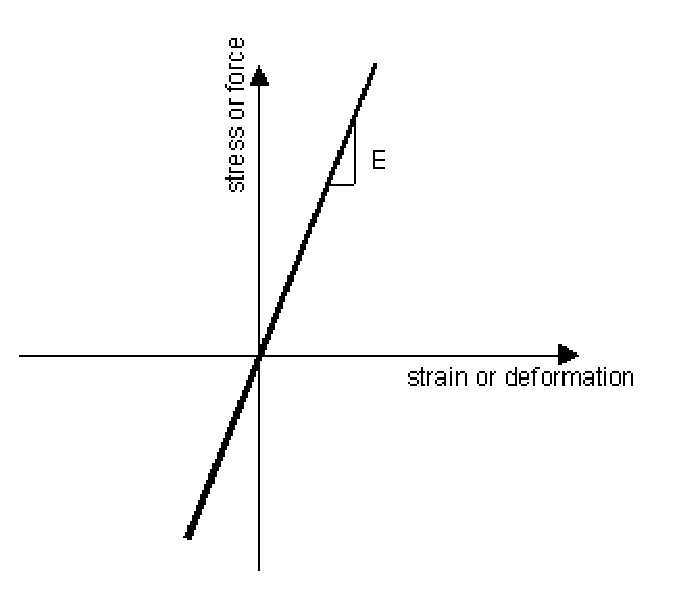
\includegraphics[width=60mm]{materials/figures/Elastic}
\caption{Elastic uniaxial material. Stress-strain diagram}\label{Elastic}
\end{figure}

\subsection{defElasticPPMaterial}
\noindent Construct an elastic perfectly-plastic uniaxial material
\begin{verbatim}
defElasticPPMaterial(mdlr,name,E,fyp,fyn)
\end{verbatim}
\vspace{-10pt}
{\color{grayLines} \rule{\linewidth}{0.25pt}}
\begin{center}
\begin{tabular}{lp{10cm}}
{\tt mdlr} & modeler name \\
{\tt name} & name identifying the material \\
{\tt E} & tangent in the elastic zone of the stress-strain diagram (see figure \ref{ElasticPP}) \\
{\tt fyp} & stress at which material reaches plastic state in tension (see figure \ref{ElasticPP}) \\
{\tt fyn} &  stress at which material reaches plastic state in compression (see figure \ref{ElasticPP}) \\
{\tt } &  \\
\end{tabular}
\end{center}
\paragraph{Example}
\begin{verbatim}
*
\end{verbatim}

\begin{figure}[h]
\centering
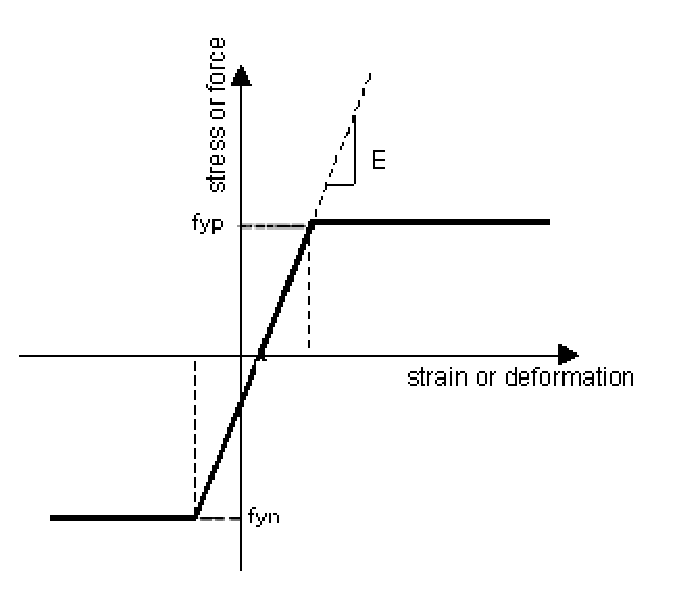
\includegraphics[width=60mm]{materials/figures/ElasticPP}
\caption{Elastic perfectly-plastic uniaxial material. Stress-strain diagram}\label{ElasticPP}
\end{figure}

\subsection{defElastNoTracMaterial}
\noindent Construct a uniaxial elastic-no tension material
\begin{verbatim}
defElastNoTracMaterial(mdlr,name,E)
\end{verbatim}
\vspace{-10pt}
{\color{grayLines} \rule{\linewidth}{0.25pt}}
\begin{center}
\begin{tabular}{lp{10cm}}
{\tt mdlr} & modeler name \\
{\tt name} & name identifying the material \\
{\tt E} & tangent in the elastic zone of the stress-strain diagram (see figure \ref{ENT}) \\
\end{tabular}
\end{center}
\paragraph{Example}
\begin{verbatim}
*
\end{verbatim}
\begin{figure}[h]
\centering
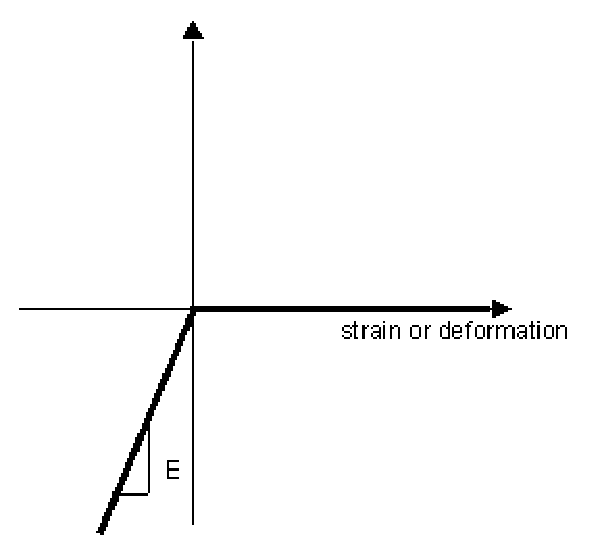
\includegraphics[width=50mm]{materials/figures/ENT}
\caption{Elastic-no tension material. Stress-strain diagram}\label{ENT}
\end{figure}

\section{Steel and reinforcing steel materials}
\subsection{defCableMaterial}
\noindent Construct a uniaxial bilinear prestressed material. The stress strain ranges from slack (large strain at zero stress) to taught (linear with modulus E).
\begin{verbatim}
defCableMaterial(mdlr,name,E,prestress,rho)
\end{verbatim}
\vspace{-10pt}
{\color{grayLines} \rule{\linewidth}{0.25pt}}
\begin{center}
\begin{tabular}{lp{10cm}}
{\tt mdlr} & modeler name \\
{\tt name} & name identifying the material \\
{\tt E} & Young modulus \\
{\tt prestress} & prestress \\
{\tt rho} & effective self weight (gravity component of weight per volume transverse to the cable) \\
\end{tabular}
\end{center}
\paragraph{Example}
\begin{verbatim}
*
\end{verbatim}


\subsection{defSteel01}
\noindent Construct a uniaxial bilinear steel material object with kinematic hardening
\begin{verbatim}
defSteel01(mdlr,name,E,fy,b)
\end{verbatim}
\vspace{-10pt}
{\color{grayLines} \rule{\linewidth}{0.25pt}}
\begin{center}
\begin{tabular}{lp{10cm}}
{\tt mdlr} & modeler name \\
{\tt name} & name identifying the material \\
{\tt E} & initial elastic tangent (see figure \ref{Steel01}) \\
{\tt fy} &  yield strength (see figure \ref{Steel01})\\
{\tt b} &  strain-hardening ratio: ratio between post-yield tangent and initial elastic tangent (see figure \ref{Steel01})\\
\end{tabular}
\end{center}
\paragraph{Example}
\begin{verbatim}
*
\end{verbatim}

\begin{figure}[h]
\centering
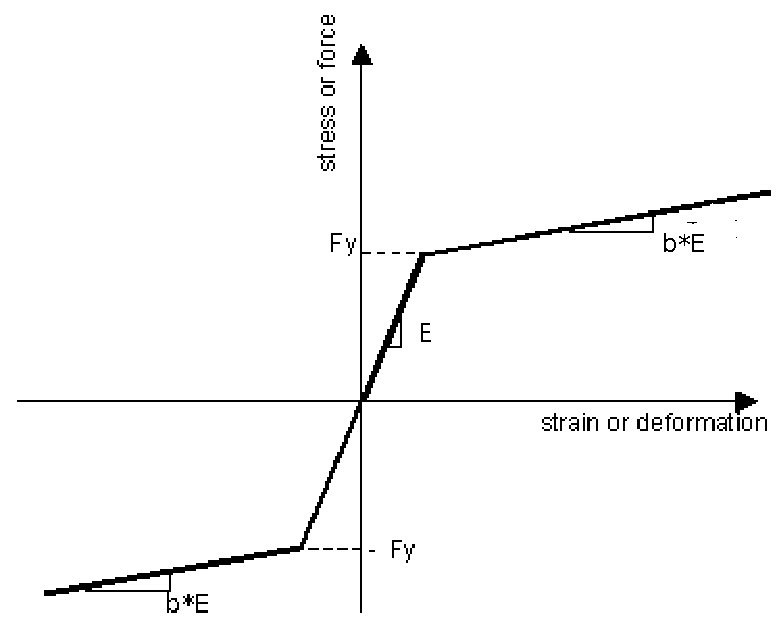
\includegraphics[width=60mm]{materials/figures/Steel01}
\caption{Steel001: uniaxial bilinear steel material with kinematic hardening. Stress-strain diagram}\label{Steel01}
\end{figure}


\subsection{defSteel02}
\noindent Construct a uniaxial Giuffre-Menegotto-Pinto steel material object with isotropic strain hardening
\begin{verbatim}
defSteel02(mdlr,name,E,fy,b,initialStress)
\end{verbatim}
\vspace{-10pt}
{\color{grayLines} \rule{\linewidth}{0.25pt}}
\begin{center}
\begin{tabular}{lp{10cm}}
{\tt mdlr} & modeler name \\
{\tt name} & name identifying the material \\
{\tt E} & initial elastic tangent (see figure \ref{Steel02}) \\
{\tt fy} &  yield strength (see figure \ref{Steel02})\\
{\tt b} &  strain-hardening ratio: ratio between post-yield tangent and initial elastic tangent)\\
{\tt initialStress} &  initial stress \\
\end{tabular}
\end{center}
{\footnotesize The transition from elastic to plastic branches  (see figure \ref{Steel02}) is controlled by parameters R0, R1, R2. The default values R0=15, R1=0.925 and R2=0.15}
\paragraph{Example}
\begin{verbatim}
*
\end{verbatim}

\begin{figure}[h]
\centering
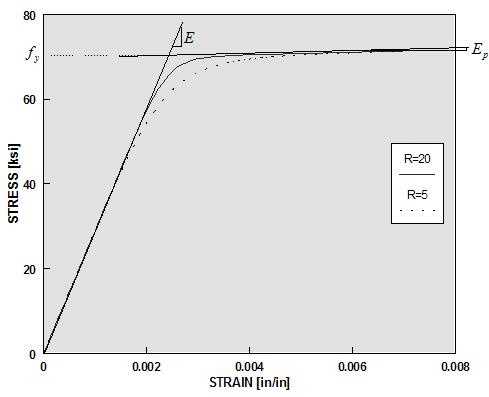
\includegraphics[width=60mm]{materials/figures/Steel02Monotonic}
\caption{Steel002: uniaxial bilinear steel material with isotropic strain hardening. Stress-strain diagram}\label{Steel02}
\end{figure}

\subsection{ReinforcingSteel}
\noindent This class constructs a bilinear stress-strain diagram to carry out the analysis of reinforced concrete according to Eurocode 2. Other national standards, like the spanish EHE and the swiss SIA also adopt this diagram.

\begin{center}
\begin{tabular}{lp{10cm}}
\multicolumn{2}{p{11cm}}{\color{grayText} \large{Parameters}} \\
\multicolumn{2}{p{13cm}}{\color{grayLines} \rule{\linewidth}{0.25pt}} \\
{\tt nmbMaterial} & name identifying the material \\
{\tt nmbDiagK} & name identifying the characteristic stress-strain diagram (default: {\tt "dgK"+nmbMaterial}) \\
{\tt tagDiagK} & tag of the uniaxial material with the characteristic stress-strain diagram\\
{\tt nmbDiagD} &  name identifying the design stress-strain diagram (default: {\tt "dgD"+nmbMaterial}) \\
{\tt tagDiagD} & tag of the uniaxial material with the design stress-strain diagram\\
{\tt fyk} & characteristic value of the yield strength\\
{\tt gammaS} & partial factor for material (default: 1.15)\\
{\tt Es} & elastic modulus of the material (default: 2e11)\\
{\tt emax} & maximum strain at failure point\\
{\tt k} & ratio between characteristic ultimate stress and characteristic yield stress $^{(1)}$ (default: 1.05)\\
\multicolumn{2}{p{13cm}}{\color{grayLines} \rule{\linewidth}{0.25pt}} \\
\multicolumn{2}{p{13cm}}{\footnotesize{(1): according to annex C of EC2: for class A k$\ge$1,05, for class B k$\ge$1,08}}
\end{tabular}
\end{center}

\begin{center}
\begin{tabular}{lp{9cm}}
\multicolumn{2}{p{11cm}}{\color{grayText} \large{Methods}} \\
\multicolumn{2}{p{13cm}}{\color{grayLines} \rule{\linewidth}{0.25pt}} \\
{\tt fmaxk()} & characteristic ultimate strength \\
{\tt fyd()} & design yield stress \\
{\tt eyk()} & characteristic strain at yield point\\
{\tt eyd()} & design strain at yield point\\
{\tt Esh()} &  post-yield tangent\\
{\tt bsh()} & ratio between post-yield tangent and initial elastic tangent\\
{\tt defDiagK(mdlr)} & returns XC uniaxial material (characteristic values)\\
{\tt defDiagD(mdlr)} & returns XC uniaxial material (design values)\\
\end{tabular}
\end{center}

\section{Concrete materials}
\subsection{defConcrete01}
\noindent Construct a uniaxial Kent-Scott-Park concrete material object with degraded linear unloading/reloading stiffness according to the work of Karsan-Jirsa and no tensile strength.
\begin{verbatim}
defConcrete01(mdlr,name,epsc0,fpc,fpcu,epscu)
\end{verbatim}
\vspace{-10pt}
{\color{grayLines} \rule{\linewidth}{0.25pt}}
\begin{center}
\begin{tabular}{lp{10cm}}
{\tt mdlr} & modeler name \\
{\tt name} & name identifying the material \\
{\tt fpc} &  concrete compressive strength at 28 days (compression is negative) $^{(1)}$\\
{\tt epsc0} &  concrete strain at maximum strength (see figure \ref{Concrete01}) $^{(2)}$\\
{\tt fpcu} &  concrete crushing strength (see figure \ref{Concrete01}) \\
{\tt epscu} &  concrete strain at crushing strength (see figure \ref{Concrete01}) \\
\hline
\multicolumn{2}{p{12cm}}{\footnotesize(1): Compressive concrete parameters should be input as negative values (if input as positive, they will be converted to negative internally)}\\
\multicolumn{2}{p{12cm}}{\footnotesize (2): The initial slope for this model is $2*fpc/epsc0$ (see figure \ref{Concrete01})}\\
\end{tabular}
\end{center}
\paragraph{Example}
\begin{verbatim}
*
\end{verbatim}

\begin{figure}[h]
\centering
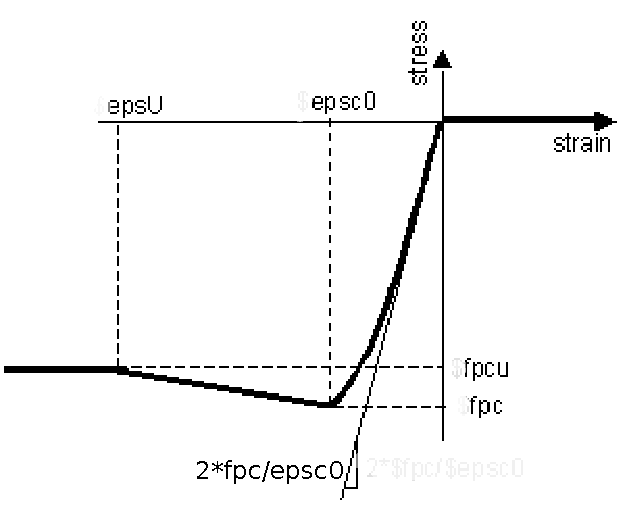
\includegraphics[width=60mm]{materials/figures/Concrete01}
\caption{Concrete01: uniaxial Kent-Scott-Park concrete material. Stress-strain diagram}\label{Concrete01}
\end{figure}

\section{ND materials}
An ND material is an object that represents the stress-strain relationship at the gauss-point of a continuum element.

\subsection{defElasticIsotropic3d}
\noindent Construct an elastic isotropic material.
\begin{verbatim}
defElasticIsotropic3d(mdlr,name,E,nu,rho)
\end{verbatim}
\vspace{-10pt}
{\color{grayLines} \rule{\linewidth}{0.25pt}}
\begin{center}
\begin{tabular}{lp{10cm}}
{\tt mdlr} & modeler name \\
{\tt name} & name identifying the material\\
{\tt E} & elastic modulus \\
{\tt nu} & Poisson's ratio \\
{\tt rho} &  mass density, optional (default = 0.0)\\
\end{tabular}
\end{center}
\paragraph{Example}
\begin{verbatim}
*
\end{verbatim}

\subsection{defElasticIsotropicPlaneStrain}
\noindent Construct an elastic isotropic plane-strain material.
\begin{verbatim}
defElasticIsotropicPlaneStrain(mdlr,name,E,nu,rho)
\end{verbatim}
\vspace{-10pt}
{\color{grayLines} \rule{\linewidth}{0.25pt}}
\begin{center}
\begin{tabular}{lp{10cm}}
{\tt mdlr} & modeler name \\
{\tt name} & name identifying the material\\
{\tt E} & elastic modulus \\
{\tt nu} & Poisson's ratio \\
{\tt rho} &  mass density, optional (default = 0.0)\\
\end{tabular}
\end{center}
\paragraph{Example}
\begin{verbatim}
*
\end{verbatim}

\subsection{defElasticIsotropicPlaneStress}
\noindent Construct an elastic isotropic plane-stress material.
\begin{verbatim}
defElasticIsotropicPlaneStress(mdlr,name,E,nu,rho)
\end{verbatim}
\vspace{-10pt}
{\color{grayLines} \rule{\linewidth}{0.25pt}}
\begin{center}
\begin{tabular}{lp{10cm}}
{\tt mdlr} & modeler name \\
{\tt name} & name identifying the material\\
{\tt E} & elastic modulus \\
{\tt nu} & Poisson's ratio \\
{\tt rho} &  mass density, optional (default = 0.0)\\
\end{tabular}
\end{center}
\paragraph{Example}
\begin{verbatim}
*
\end{verbatim}
\section{Sections}
A section represents a force-deformation (or resultant stress-strain) relationship at beam-column or plate element.

Three types of sections are going to be considered:
\begin{description}
\item{Elastic:} defined by material and geometric constants;
\item{Resultant:} general nonlinear description of force-deformation response, e.g. moment-curvature;
\item{Fiber:} section is discretized into smaller regions for which the material stress-strain response is integrated to give resultant behavior, e.g. reinforced concrete.
\end{description}
\subsection{Elastic sections}
\subsubsection{defElasticSection2d}
\noindent Construct an elastic section appropiate for 2D beam analysis.
\begin{verbatim}
defElasticSection2d(mdlr,name,A,E,I)
\end{verbatim}
\vspace{-10pt}
{\color{grayLines} \rule{\linewidth}{0.25pt}}
\begin{center}
\begin{tabular}{lp{10cm}}
{\tt mdlr} & modeler name \\
{\tt name} & name identifying the section \\
{\tt A} &  cross-sectional area of the section \\
{\tt E} &  Young's modulus of material \\
{\tt I} &  second moment of area about the local z-axis\\
\end{tabular}
\end{center}
\paragraph{Example}
\begin{verbatim}
*
\end{verbatim}


\subsubsection{defElasticShearSection2d}
\noindent Construct an elastic section appropiate for 2D beam analysis, including shear deformations.
\begin{verbatim}
defElasticShearSection2d(mdlr,name,A,E,G,I,alpha)
\end{verbatim}
\vspace{-10pt}
{\color{grayLines} \rule{\linewidth}{0.25pt}}
\begin{center}
\begin{tabular}{lp{10cm}}
{\tt mdlr} & modeler name \\
{\tt name} & name identifying the section \\
{\tt A} &  cross-sectional area of the section \\
{\tt E} &  Young's modulus of material \\
{\tt G} & shear modulus \\
{\tt I} &  second moment of area about the local z-axis\\
{\tt alpha} & shear shape factor \\
\end{tabular}
\end{center}
\paragraph{Example}
\begin{verbatim}
*
\end{verbatim}

\subsubsection{defElasticSectionFromMechProp2d}
\noindent Construct an elastic section appropiate for 2D beam analysis, taking mechanical properties of the section form a MechProp2d object.
\begin{verbatim}
defElasticSectionFromMechProp2d(mdlr,name,mechProp2d)
\end{verbatim}
\vspace{-10pt}
{\color{grayLines} \rule{\linewidth}{0.25pt}}
\begin{center}
\begin{tabular}{lp{10cm}}
{\tt mdlr} & modeler name \\
{\tt name} & name identifying the section \\
{\tt mechProp2d} & object that contains mechanical properties of the section  \\
\end{tabular}
\end{center}
\paragraph{Example}
\begin{verbatim}
*
\end{verbatim}

%%%
\subsubsection{defElasticSection3d}
\noindent Construct an elastic section appropiate for 3D beam analysis.
\begin{verbatim}
defElasticSection3d(mdlr,name,A,E,G,Iz,Iy,J)
\end{verbatim}
\vspace{-10pt}
{\color{grayLines} \rule{\linewidth}{0.25pt}}
\begin{center}
\begin{tabular}{lp{10cm}}
{\tt mdlr} & modeler name \\
{\tt name} & name identifying the section \\
{\tt A} &  cross-sectional area of the section \\
{\tt E} &  Young's modulus of material \\
{\tt Iz} &  second moment of area about the local z-axis\\
{\tt Iy} &  second moment of area about the local y-axis\\
{\tt J} & torsional moment of inertia of the section \\
\end{tabular}
\end{center}
\paragraph{Example}
\begin{verbatim}
*
\end{verbatim}


\subsubsection{defElasticShearSection3d}
\noindent Construct an elastic section appropiate for 3D beam analysis, including shear deformations.
\begin{verbatim}
defElasticShearSection3d(mdlr,name,A,E,G,Iz,Iy,J,alpha)
\end{verbatim}
\vspace{-10pt}
{\color{grayLines} \rule{\linewidth}{0.25pt}}
\begin{center}
\begin{tabular}{lp{10cm}}
{\tt mdlr} & modeler name \\
{\tt name} & name identifying the section \\
{\tt A} &  cross-sectional area of the section \\
{\tt E} &  Young's modulus of material \\
{\tt G} & shear modulus \\
{\tt Iz} &  second moment of area about the local z-axis\\
{\tt Iy} &  second moment of area about the local y-axis\\
{\tt J} & torsional moment of inertia of the section \\
{\tt alpha} & shear shape factor \\
\end{tabular}
\end{center}
\paragraph{Example}
\begin{verbatim}
*
\end{verbatim}

\subsubsection{defElasticSectionFromMechProp3d}
\noindent Construct an elastic section appropiate for 3D beam analysis, taking mechanical properties of the section form a MechProp3d object.
\begin{verbatim}
defElasticSectionFromMechProp3d(mdlr,name,mechProp3d)
\end{verbatim}
\vspace{-10pt}
{\color{grayLines} \rule{\linewidth}{0.25pt}}
\begin{center}
\begin{tabular}{lp{10cm}}
{\tt mdlr} & modeler name \\
{\tt name} & name identifying the section \\
{\tt mechProp3d} & object that contains mechanical properties of the section  \\
\end{tabular}
\end{center}
\paragraph{Example}
\begin{verbatim}
*
\end{verbatim}

\subsubsection{defElasticMembranePlateSection}
\noindent Construct an an isotropic elastic section appropriate for plate and shell analysis.
\begin{verbatim}
defElasticMembranePlateSection(mdlr,name,E,nu,rho,h)
\end{verbatim}
\vspace{-10pt}
{\color{grayLines} \rule{\linewidth}{0.25pt}}
\begin{center}
\begin{tabular}{lp{10cm}}
{\tt mdlr} & modeler name \\
{\tt name} & name identifying the section\\
{\tt E} &  Young's modulus\\
{\tt nu} &  Poisson's modulus\\
{\tt rho} &  mass density\\
{\tt h} &  depth of section\\
\end{tabular}
\end{center}
\paragraph{Example}
\begin{verbatim}
*
\end{verbatim}

\subsubsection{defElasticPlateSection}
\noindent Construct an an isotropic elastic section appropriate for plate analysis.
\begin{verbatim}
defElasticPlateSection(mdlr,name,E,nu,rho,h)
\end{verbatim}
\vspace{-10pt}
{\color{grayLines} \rule{\linewidth}{0.25pt}}
\begin{center}
\begin{tabular}{lp{10cm}}
{\tt mdlr} & modeler name \\
{\tt name} & name identifying the section\\
{\tt E} &  Young's modulus\\
{\tt nu} &  Poisson's modulus\\
{\tt rho} &  mass density\\
{\tt h} &  depth of section\\
\end{tabular}
\end{center}
\paragraph{Example}
\begin{verbatim}
*
\end{verbatim}

\subsection{Fiber sections}
\subsubsection{FiberSet}
\noindent This class constructs a set of fibers for a fiber section
\begin{verbatim}
FiberSet(scc,nmbSet,tagDiag)
\end{verbatim}
\begin{center}
\begin{tabular}{lp{10cm}}
\multicolumn{2}{p{11cm}}{\color{grayText} \large{Parameters}} \\
\multicolumn{2}{p{13cm}}{\color{grayLines} \rule{\linewidth}{0.25pt}} \\
{\tt scc} & name identifying the fiber section \\
{\tt nmbSet} & name of the set of fibers to be generated \\
{\tt tagDiag} & tag of the uniaxial material which forms the fibers \\
\end{tabular}
\end{center}

\begin{center}
\begin{tabular}{lp{9cm}}
\multicolumn{2}{p{11cm}}{\color{grayText} \large{Methods}} \\
\multicolumn{2}{p{13cm}}{\color{grayLines} \rule{\linewidth}{0.25pt}} \\
{\tt getFiberWithMinStrain()} & returns the fiber of the set that has the minimum strain \\
{\tt getFiberWithMaxStrain()} & returns the fiber of the set that has the maximum strain \\
\end{tabular}
\end{center}


\subsubsection{RCSets}
\noindent This class constructs the sets (concrete and reinforcing steel) of a reinforced concrete fiber section.
\begin{verbatim}
RCSets(scc,tagCdiag, nmbSetC,tagSdiag, nmbSetS)
\end{verbatim}
\begin{center}
\begin{tabular}{lp{10cm}}
\multicolumn{2}{p{11cm}}{\color{grayText} \large{Parameters}} \\
\multicolumn{2}{p{13cm}}{\color{grayLines} \rule{\linewidth}{0.25pt}} \\
{\tt scc} & name identifying the fiber section \\
{\tt tagCDiag} & tag of the uniaxial material that makes up the concrete fibers of the section \\
{\tt nmbSetC} & name of the set of fibers of concrete to be generated \\
{\tt tagSdiag} & tag of the uniaxial material that makes up the reinforcing steel fibers of the section \\
{\tt nmbSetS} & name of the set of fibers of reinforcing steel to be generated \\
\end{tabular}
\end{center}

\begin{center}
\begin{tabular}{lp{9cm}}
\multicolumn{2}{p{11cm}}{\color{grayText} \large{Methods}} \\
\multicolumn{2}{p{13cm}}{\color{grayLines} \rule{\linewidth}{0.25pt}} \\
{\tt reselTractionFibers(scc,tractionFibersSetName)} & returns the set of fibers in tension \\
{\tt getConcreteArea(factor)} & returns the concrete area \\
{\tt getMaxConcreteStrain()} & returns the maximum strain in the set of concrete fibers \\
{\tt getConcreteInitialTangent()} & returns the initial tangent in the stress-strain diagram of material that makes up the fibers of concrete \\
{\tt getConcreteCompression()} & returns the resultant of compressive stresses in concrete fibers \\
{\tt getNumBarrasTraccion()} & returns the number of reinforcing steel fibers in tension \\
\end{tabular}
\end{center}

\subsubsection{fiberSectionSetupRCSets}
Returns an object of the class \verb|RCSets|
\begin{verbatim}
fiberSectionSetupRCSets(scc,tagCdiag, nmbSetC,tagSdiag, nmbSetS)
\end{verbatim}
\vspace{-10pt}
{\color{grayLines} \rule{\linewidth}{0.25pt}}
\begin{center}
\begin{tabular}{lp{10cm}}
{\tt scc} & name identifying the fiber section \\
{\tt tagCdiag} & tag of the uniaxial material that makes up the concrete fibers of the section \\
{\tt nmbSetC} & name of the set of fibers of concrete to be generated \\
{\tt tagSdiag} & tag of the uniaxial material that makes up the reinforcing steel fibers of the section \\
{\tt nmbSetS} & name of the set of fibers of reinforcing steel to be generated \\
\end{tabular}
\end{center}

\subsubsection{creaSetsFibrasHA}
Construct the sets of concrete fibers (\verb|"hormigon"|) and reinforcing steel fibers (\verb|"armadura"|) for all the elements included in a set of elements.
\begin{verbatim}
creaSetsFibrasHA(mdlr, nmbSet, tagHA, tagAcero)
\end{verbatim}
\vspace{-10pt}
{\color{grayLines} \rule{\linewidth}{0.25pt}}
\begin{center}
\begin{tabular}{lp{10cm}}
{\tt mdlr} & modeler name \\
{\tt nmbSet} & name identifying the set of elements \\
{\tt tagHA} & tag of the uniaxial material that makes up the concrete fibers of the section \\
{\tt tagAcero} & tag of the uniaxial material that makes up the reinforcing steel fibers of the section \\
\end{tabular}
\end{center}

\subsubsection{reselTractionFibers}
Returns the fibers under tension included in a set of fibers.
\begin{verbatim}
reselTractionFibers(scc,fiberSetName,tractionFibersSetName)
\end{verbatim}
\vspace{-10pt}
{\color{grayLines} \rule{\linewidth}{0.25pt}}
\begin{center}
\begin{tabular}{lp{10cm}}
{\tt scc} & name identifying the fiber section \\
{\tt fiberSetName} & name identifying the set of fibers \\
{\tt tractionFibersSetName} & name of the set of tensioned fibers returned\\
\end{tabular}
\end{center}

\subsubsection{fiberSectionSetupRC3Sets}
Returns a set of tensioned fibers (\verb|"armaduraTraccion"|) of a fiber section of reinforced concrete.
\begin{verbatim}
fiberSectionSetupRC3Sets(scc,tagCdiag, nmbSetC,tagSdiag, nmbSetS)
\end{verbatim}
\vspace{-10pt}
{\color{grayLines} \rule{\linewidth}{0.25pt}}
\begin{center}
\begin{tabular}{lp{10cm}}
{\tt scc} & name identifying the fiber section \\
{\tt tagCdiag} & tag of the uniaxial material that makes up the concrete fibers of the section \\
{\tt nmbSetC} & name of the set of fibers of concrete to be generated \\
{\tt tagSdiag} & tag of the uniaxial material that makes up the reinforcing steel fibers of the section \\
{\tt nmbSetS} & name of the set of fibers of reinforcing steel to be generated \\
\end{tabular}
\end{center}

\subsubsection{RecordSeccionHAPilar}
\noindent This class is used to define the variables that make up a reinforced concrete section with reinforcement symmetric in both directions (as usual in columns)
\begin{verbatim}
RecordSeccionHAPilar()
\end{verbatim}
\begin{center}
\begin{tabular}{lp{10cm}}
\multicolumn{2}{p{11cm}}{\color{grayText} \large{Parameters}} \\
\multicolumn{2}{p{13cm}}{\color{grayLines} \rule{\linewidth}{0.25pt}} \\
{\tt nmbSeccion} & name identifying the section \\
{\tt descSeccion} & section description \\
{\tt nmbGeomSeccion} & name identifying the geometric section \\
{\tt tipoHormigón} & type of concrete (e.g. hormigonesEHE.HA25) \\
{\tt nmbDiagHormigon} & name identifying the characteristic stress-strain diagram of the concrete material \\
{\tt canto} & cross-section height \\
{\tt ancho} & cross-section width \\
{\tt numDivIJ} & number of cells in IJ (width) direction \\
{\tt numDivJK} & number of cells in JK  (height) direction \\
{\tt tipoArmadura} & type of reinforcement steel \\
{\tt nmbDiagArmadura} & name identifying the characteristic stress-strain diagram of the reinforcing steel material \\
{\tt recub} & cover \\
{\tt nBarrasAncho} & number of rebars in the width direction of the section (each face)\\
{\tt areaBarrasAncho} & area of each rebar in  width direction \\
{\tt nBarrasCanto} & number of rebars in the height direction of the section (each face )\\
{\tt areaBarrasCanto} & area of each rebar in height direction \\
{\tt armCortanteZ} & record of type {\tt defSeccionHASimple.RecordArmaduraCortante()} defining the shear reinforcement in Z direction \\
{\tt armCortanteY} & record of type {\tt defSeccionHASimple.RecordArmaduraCortante()} defining the shear reinforcement in Y direction \\
\end{tabular}
\end{center}

\begin{center}
\begin{tabular}{lp{9cm}}
\multicolumn{2}{p{11cm}}{\color{grayText} \large{Methods}} \\
\multicolumn{2}{p{13cm}}{\color{grayLines} \rule{\linewidth}{0.25pt}} \\
{\tt defGeomSeccHAPilar(tipoDiag)} & returns a reinforced concrete section with reinforcement symmetric in both directions \\
& {\tt tipoDiag} ="k" for characteristic diagram, ="d" for design diagram \\ 
\end{tabular}
\end{center}


\subsubsection{Utils}
\paragraph{Module materials.regimenSeccion}
\subparagraph{tipoSolicitacion}
\noindent Returns the following values, depending on the state of stress in the section:
\begin{description}
\item{1} pure or combined tension where the entire section is under tension;
\item{2} pure or combined bending (there are fibres in tension and in compression);
\item{3} single or combined compression where all the fibres are in compression.
\end{description}
\begin{verbatim}
tipoSolicitacion(epsCMin, epsSMax)
\end{verbatim}
\vspace{-10pt}
{\color{grayLines} \rule{\linewidth}{0.25pt}}
\begin{center}
\begin{tabular}{lp{10cm}}
{\tt epsCMin} & minimum strain in concrete \\
{\tt epsSMax} & maximum strain in steel \\
\end{tabular}
\end{center}

\subparagraph{strTipoSolicitacion}
\noindent Returns:
\begin{description}
\item{\verb|"tracción simple o compuesta"|} in pure or combined tension state;
\item{\verb|"flexotracción"|} in pure or combined bending state;
\item{\verb|"compresión simple o compuesta"|} in single or combined compression state;
\item{\verb|"falla"|} in all other cases.
\end{description}
\begin{verbatim}
strTipoSolicitacion(tipoSol)
\end{verbatim}
\vspace{-10pt}
{\color{grayLines} \rule{\linewidth}{0.25pt}}
\begin{center}
\begin{tabular}{lp{10cm}}
{\tt tipoSol} & =1 for pure or combined tension state \\
& =2 for pure or combined bending state \\
& =3 for single or combined compression state \\
\end{tabular}
\end{center}







\end{document}




\subsection{}
\noindent 
\begin{verbatim}

\end{verbatim}
\vspace{-10pt}
{\color{grayLines} \rule{\linewidth}{0.25pt}}
\begin{center}
\begin{tabular}{lp{10cm}}
{\tt mdlr} & modeler name \\
{\tt name} & name identifying the \\
{\tt } &  \\
{\tt } &  \\
{\tt } &  \\
\end{tabular}
\end{center}
\paragraph{Example}
\begin{verbatim}
*
\end{verbatim}

\begin{figure}[h]
\centering
\includegraphics[width=60mm]{materials/figures/}
\caption{. Stress-strain diagram}\label{}
\end{figure}


\chapter{Elements}

\section{Zero-length elements}
\subsection{ZeroLength}
The ZeroLength class represents an element defined by two nodes at the same geometric location, hence it has zero length.

The nodes are connected by means of uniaxial materials to represent the force-deformation relationship for the element. 

ZeroLength elements are constructed with a {\em tag} in a domain of {\em dimension} 1, 2, or 3, connected by nodes {\em Nd1} and {\em Nd2}. 
The vector $\vec{x}$ defines the local x-axis for the element and the vector $\vec{yp}$ lies in the local x-y plane for the element.  The local z-axis is the cross product between $\vec{x}$ and $\vec{yp}$, and the local y-axis is the cross product between the local z-axis and $\vec{x}$.

The force-deformation relationship for the element is given by a pointer {\em theMaterial} to a {\bf UniaxialMaterial} model acting in local {\em direction}.

The local {\em direction} is 0, 1, 2 for translation in the local x, y, z axes or 3, 4, 5 for rotation about the local x, y, z axes. 

\begin{verbatim}
mdlr=xc.ProblemaEF().getModelador
ZeroLengthElement=mdlr.getElementLoader.newElement("zero_length",
xc.ID([Nd1Tag,Nd2Tag]))
\end{verbatim}
\begin{paramFuncTable}
{\tt Nd1Tag,Nd2Tag} & tags of the nodes connected by the element\\
\end{paramFuncTable}

\begin{paramClassTable}
\ElementParam{}
\ElementZERODParam{}
\end{paramClassTable}

\begin{methodsTable}
\ElementMeth{}
\ElementZERODMeth{}
\ZeroLengthMeth{}
\end{methodsTable}

% ***ZeroLengthSection***
\subsection{ZeroLengthSection}
The ZeroLengthSection class represents an element defined by two nodes at the same geometric location, hence it has zero length.

The nodes are connected by a SectionForceDeformation object which represents the force-deformation relationship for the element. 

ZeroLength elements are constructed with a {\em tag} in a domain of {\em dimension} 1, 2, or 3, connected by nodes {\em Nd1} and {\em Nd2}. 
The vector $\vec{x}$ defines the local x-axis for the element and the vector $\vec{yp}$ lies in the local x-y plane for the element.  The local z-axis is the cross product between $\vec{x}$ and $\vec{yp}$, and the local y-axis is the cross product between the local z-axis and $\vec{x}$.

The force-deformation relationship for the element is obtained by invoking {\em getCopy()} on the {\bf SectionForceDeformation} pointer {\em theSection}. The section model acts in the local space defined by the $\vec{x}$ and $\vec{yp}$ vectors. The section axial force-deformation acts along the element local x-axis and the section y-z axes directly corresponds to the local element y-z axes.

\begin{verbatim}
mdlr=xc.ProblemaEF().getModelador
ZeroLengthElement=mdlr.getElementLoader.newElement(
"zero_length_section",xc.ID([Nd1Tag,Nd2Tag]))
\end{verbatim}
\begin{paramFuncTable}
{\tt Nd1Tag,Nd2Tag} & tags of the nodes connected by the element\\
\end{paramFuncTable}

\begin{paramClassTable}
\ElementParam{}
\ElementZERODParam{}
\end{paramClassTable}

\begin{methodsTable}
\ElementMeth{}
\ElementZERODMeth{}
\ZeroLengthSectionMeth{}
\end{methodsTable}


\subsection{ZeroLengthContact2D, ZeroLengthContact3D}
% ***ZeroLengthContact***
These classes are used to construct a zeroLengthContact2D element or a zeroLengthContact3D element, which are Node-to-node frictional contact element used in two dimensional analysis and three dimensional analysis.

The contact element is node-to-node contact. Contact occurs between two contact nodes when they come close. The relation follows Mohr-coulomb law: $T = \mu \cdot N + c$, where $T$ is tangential force and $N$ is normal force across the interface; $\mu$ is friction coefficient and $c$ is total cohesion (summed over the effective area of contact nodes).

The contact node pair in node-to-node contact element is termed «master node» and «slave node», respectively. Master/slave plane is the contact plane which the master/slave node belongs to. The discrimination is made solely for contact detection purpose. User need to specify the corresponding out normal of the master plane, and this direction is assumed to be unchanged during analysis. For simplicity, 3D contact only allows 3 options to specify the directions of the contact plane. The convention is: out normal of master plane always points to positive axial direction (+X or +Y, or +Z)

For 2D contact, slave nodes and master nodes must be 2 DOF. For 3D contact, slave nodes and master nodes must be 3 DOF.

The resulted tangent from the contact element is non-symmetric. Switch to non-symmetric matrix solver. 

\begin{verbatim}
mdlr=xc.ProblemaEF().getModelador
ZeroLengthElement=mdlr.getElementLoader.newElement(
"zero_length_contact_2d",xc.ID([Nd1Tag,Nd2Tag]))
"zero_length_contact_3d",xc.ID([Nd1Tag,Nd2Tag]))
\end{verbatim}
\begin{paramFuncTable}
{\tt Nd1Tag,Nd2Tag} & tags of master and slave nodes\\
\end{paramFuncTable}


\begin{paramClassTable}
\ElementParam{}
\ElementZERODParam{}
\end{paramClassTable}

\begin{methodsTable}
\ElementMeth{}
\ElementZERODMeth{}
\end{methodsTable}



\section{Truss elements}

% ***Truss***
\subsection{Truss}
This class is used to construct a truss element object defined by two nodes connected by means of a previously defined uniaxial material.
The truss element does not include geometric nonlinearities, even when used with beam-columns utilizing P-Delta or Corotational transformations.
The truss element considers strain-rate effects, and is thus suitable for use as a damping element. 
\begin{verbatim}
mdlr=xc.ProblemaEF().getModelador
trussElement=mdlr.getElementLoader.newElement(
"truss",xc.ID([Nd1Tag,Nd2Tag]))
\end{verbatim}
\begin{paramFuncTable}
{\tt Nd1Tag,Nd2Tag} & tags of the nodes connected by the element\\
\end{paramFuncTable}

\begin{paramClassTable}
\ElementParam{}
\ElementOneDParam{}
\end{paramClassTable}

\begin{methodsTable}
\ElementMeth{}
\ElementOneDMeth{}
\ProtoTrussMeth{}
\TrussBaseMeth{}
\TrussMeth{}
\end{methodsTable}


% ***TrussSection***
\subsection{TrussSection}
This class is used to construct a truss element object defined by two nodes connected by means of a previously defined section.
\begin{verbatim}
mdlr=xc.ProblemaEF().getModelador
trussSectionElement=mdlr.getElementLoader.newElement(
"truss_section",xc.ID([Nd1Tag,Nd2Tag]))
\end{verbatim}
\begin{paramFuncTable}
{\tt Nd1Tag,Nd2Tag} & tags of the nodes connected by the element\\
\end{paramFuncTable}

\begin{paramClassTable}
\ElementParam{}
\ElementOneDParam{}
\end{paramClassTable}

\begin{methodsTable}
\ElementMeth{}
\ElementOneDMeth{}
\ProtoTrussMeth{}
\TrussBaseMeth{}
\end{methodsTable}

% ***CorotTruss***
\subsection{CorotTruss}
This class is used to construct a corotational truss element object defined by two nodes connected by means of a previously defined uniaxial material.

When constructed with a UniaxialMaterial object, the corotational truss element considers strain-rate effects, and is thus suitable for use as a damping element.
\begin{verbatim}
mdlr=xc.ProblemaEF().getModelador
corotTrussElement=mdlr.getElementLoader.newElement(
"corot_truss",xc.ID([Nd1Tag,Nd2Tag]))
\end{verbatim}
\begin{paramFuncTable}
{\tt Nd1Tag,Nd2Tag} & tags of the nodes connected by the element\\
\end{paramFuncTable}

\begin{paramClassTable}
\ElementParam{}
\ElementOneDParam{}
\CorotTrussParam{}
\end{paramClassTable}

\begin{methodsTable}
\ElementMeth{}
\ElementOneDMeth{}
\ProtoTrussMeth{}
\CorotTrussMeth{}
\end{methodsTable}

% ***CorotTrussSection***
\subsection{CorotTrussSection}
This class is used to construct a corotational truss element object defined by two nodes connected by means of a previously defined section.

\begin{verbatim}
mdlr=xc.ProblemaEF().getModelador
corotTrussSectionElement=mdlr.getElementLoader.newElement(
"corot_truss_section",xc.ID([Nd1Tag,Nd2Tag]))
\end{verbatim}
\begin{paramFuncTable}
{\tt Nd1Tag,Nd2Tag} & tags of the nodes connected by the element\\
\end{paramFuncTable}

\begin{paramClassTable}
\ElementParam{}
\ElementOneDParam{}
\end{paramClassTable}

\begin{methodsTable}
\ElementMeth{}
\ElementOneDMeth{}
\ProtoTrussMeth{}
\end{methodsTable}

\section{Beam-column elements}

% ***ElasticBeam2d***
\subsection{ElasticBeam2d}
This class is used to construct a uniaxial element with tension, compression, and bending capabilities. The element has three degrees of freedom at each node: translations in the nodal x and y directions and rotation about the nodal z-axis.

The element is defined by two 2D nodes, a previously-defined coordinate-transformationt object and a previously-defined 2D elastic section. The initial strain in the element (initialStrain) is given by $\Delta/L$, where $\Delta$ is the difference between the element length, L (as defined by the 1 and 2 node locations), and the zero strain length. 

\begin{verbatim}
mdlr=xc.ProblemaEF().getModelador
elasticBeam2dElement=mdlr.getElementLoader.newElement(
"elastic_beam_2d",xc.ID([Nd1Tag,Nd2Tag]))
\end{verbatim}
\begin{paramFuncTable}
{\tt Nd1Tag,Nd2Tag} & tags of the nodes connected by the element\\
\end{paramFuncTable}

\begin{paramClassTable}
\ElementParam{}
\ElementOneDParam{}
\ProtoBeamTwoDParam{}
\rhoX{} \\
\h{}  \\
\initialStrain{} \\
\getV{} \\
\getVOne{} \\
\getVTwo{} \\
\getNOne{} \\
\getNTwo{} \\
\getMOne{} \\
\getMTwo{} \\
\end{paramClassTable}

\begin{methodsTable}
\ElementMeth{} 
\ElementOneDMeth{}
\end{methodsTable}

% ***ElasticBeam3d***
\subsection{ElasticBeam3d}
This class is used to construct a uniaxial element with tension, compression, torsion, and bending capabilities. The element has six degrees of freedom at each node: translations in the nodal x, y, and z directions and rotations about the nodal x, y, and z axes. 

The element is defined by two 3D nodes, a previously-defined coordinate-transformationt object and a previously-defined 3D elastic section. The element x-axis is oriented from node I toward node J. The initial strain in the element (initialStrain) is given by $\Delta/L$, where $\Delta$ is the difference between the element length, L (as defined by the 1 and 2 node locations), and the zero strain length. 

\begin{verbatim}
mdlr=xc.ProblemaEF().getModelador
elasticBeam2dElement=mdlr.getElementLoader.newElement(
"elastic_beam_3d",xc.ID([Nd1Tag,Nd2Tag]))
\end{verbatim}
\begin{paramFuncTable}
{\tt Nd1Tag,Nd2Tag} & tags of the nodes connected by the element\\
\end{paramFuncTable}


\begin{paramClassTable}
\ElementParam{}
\ElementOneDParam{}
\ProtoBeamThreeDParam{}
\rhoX{} \\
\initialStrain{} \\
\getANTwo{} \\
\getNOne{} \\
\getNTwo{} \\
\getN{} \\
\getAMzOne{} \\
\getAMzTwo{} \\
\getMzOne{} \\
\getMzTwo{} \\
\getMyOne{} \\
\getMyTwo{} \\
\getVy{} \\
\getVyOne{} \\
\getVyTwo{} \\
\getAVyOne{} \\
\getAVyTwo{} \\
\getVz{} \\
\getVzOne{} \\
\getVzTwo{} \\
\getAVzOne{} \\
\getAVzTwo{} \\
\end{paramClassTable}

\begin{methodsTable}
\ElementMeth{}
\ElementOneDMeth{}
\getVDirEjeFuerteLocales{} \\
\getVDirEjeDebilLocales{} \\
\getAnguloEjeFuerte{} \\
\getAnguloEjeDebil{} \\
\getVDirEjeFuerteGlobales{} \\
\getVDirEjeDebilGlobales{} \\

\end{methodsTable}

% ***ForceBeamColumn2d***
\subsection{ForceBeamColumn2d}
This command is used to construct a 2D forceBeamColumn element object, which is based on the iterative force-based formulation. A variety of numerical integration options can be used in the element state determination and encompass both distributed plasticity and plastic hinge integration. More details on the available numerical integration options can be found in the paper titled «Numerical Integration Options for the Force-Based Beam-Column Element in OpenSees», by Michael H. Scott.

The element is defined by two 2D nodes, a previously-defined coordinate-transformationt object and a previously-defined 2D elastic section.
\begin{verbatim}
mdlr=xc.ProblemaEF().getModelador
elasticBeam2dElement=mdlr.getElementLoader.newElement(
"force_beam_column_2d",xc.ID([Nd1Tag,Nd2Tag]))
\end{verbatim}
\begin{paramFuncTable}
{\tt Nd1Tag,Nd2Tag} & tags of the nodes connected by the element\\
\end{paramFuncTable}

\begin{paramClassTable}
\ElementParam{}
\ElementOneDParam{}
\rhoX{}
\end{paramClassTable}

\begin{methodsTable}
\ElementMeth{}
\ElementOneDMeth{}
\BeamColumnWithSectionFDMeth{}
\end{methodsTable}

% ***ForceBeamColumn3d***
\subsection{ForceBeamColumn3d}
This command is used to construct a 3D forceBeamColumn element object, which is based on the iterative force-based formulation. A variety of numerical integration options can be used in the element state determination and encompass both distributed plasticity and plastic hinge integration. More details on the available numerical integration options can be found in the paper titled «Numerical Integration Options for the Force-Based Beam-Column Element in OpenSees», by Michael H. Scott. 

The element is defined by two 3D nodes, a previously-defined coordinate-transformationt object and a previously-defined 3D elastic section.
\begin{verbatim}
mdlr=xc.ProblemaEF().getModelador
elasticBeam2dElement=mdlr.getElementLoader.newElement(
"force_beam_column_3d",xc.ID([Nd1Tag,Nd2Tag]))
\end{verbatim}
\begin{paramFuncTable}
{\tt Nd1Tag,Nd2Tag} & tags of the nodes connected by the element\\
\end{paramFuncTable}
\begin{paramClassTable}
\ElementParam{}
\ElementOneDParam{}
\rhoX{}
\end{paramClassTable}

\begin{methodsTable}
\ElementMeth{}
\ElementOneDMeth{}
\BeamColumnWithSectionFDMeth{}
\getVDirEjeFuerteLocales{} \\
\getVDirEjeDebilLocales{} \\
\getAnguloEjeFuerte{} \\
\getAnguloEjeDebil{} \\
\getVDirEjeFuerteGlobales{} \\
\getVDirEjeDebilGlobales{} \\
\end{methodsTable}

\chapter{Model}
\section{Index of variable names}
This section includes those names which are most often used in this chapter for designing parameters. 
\begin{center}
\begin{tabular}{lp{10cm}}
{\tt mdlr} & modeler name (see \ref{getModelador})\\


\end{tabular}
\end{center}


\section{ProblemaEF}
\begin{verbatim}
import xc_base
import xc
xc.ProblemaEF()
\end{verbatim}

\section{getModelador}\label{getModelador}
Modeler
\begin{verbatim}
import xc_base
import xc
mdlr=xc.ProblemaEF().getModelador
\end{verbatim}

\section{getModelador}\label{getModelador}
Points container
\begin{verbatim}
import xc_base
import xc
points=mdlr.getCad.getPoints
\end{verbatim}




\appendix
\chapter{Generation of combinations to consider in the structural calculation}

\section{Introduction}
This Appendix has the object of defining the actions, weighting coefficients and the combination of actions which shall be taken into account when designing structures.

Checking the structures through design is the most used method to guarantee their safety \footnote{Other procedures are also acceptable such as the reduced model tests, full-scale tests of the structure or its elements, extrapolation of the behaviour of similar structures, \ldots}.

\subsection{The Limit States design method} \label{limit_states_introd}
The usual method prescribed by the codes for checking the safety of a structure is the so-called \emph{Method of limit states}. A \emph{limit state} is a situation in which, when exceeded, it may be considered that the structure does not fulfil one of the functions for which it has been designed.

The limit states are classified in:
\begin{itemize}
\item \emph{Ultimate Limit States (ULS)};
\item \emph{Serviceability Limit States (SLS)}, and
\item \emph{Durability Limit States (DLS)}.
\end{itemize}

\subsection{Design situations}
The concept of \emph{design situation} is useful to sort the checks performed on the project or study of a structure. A design situation is a simplified representation of the reality that is amenable to analysis.

Thus, it can be considered design situations those that correspond to the different phases of construction of the structure, the normal use of the structure, its reparation, exceptional conditions, \ldots. 

For each of the design situations, it must be checked that the structure doesn't exceed any of the Limit States previously laid down in paragraph \ref{limit_states_introd}

\subsection{Actions}
\emph{Action} is defined as any cause capable of producing stress states in a structure, or modifying the existing one. Weight coefficients can be different according to the codes that apply for verification of the different structural elements (IAP, EHE, Eurocodes,\ldots).

\subsection{Working life} \label{sc_vida_util}
The working life of a structure is the period of time from the end of its execution, during which must maintain the requirements of security and functionality of project and an acceptable aesthetic appearance. During that period it will require conservation in accordance with the maintenance plan established for that purpose.

The design working life depends on the type of structure and must be fixed by the Owners at the start of the design. In any case its duration will be lower than that indicated in the regulations applicable or, in the absence of these, than the values laid down in Table \ref{tb_vid_util}.


\begin{table}
\begin{center}
\begin{small}
\begin{tabular}{|p{6cm}|l|}
\hline
\textbf{Type of structure} & \textbf{Design working life} \\
\hline
Temporary structures (*) & 3 to 10 years (*) \\
\hline
Replaceable structural elements that are not part of the main structure (eg, handrails, pipe supports) & 10 to 25 years \\
\hline
Agricultural or industrial buildings (or installations) and maritime works & 15 to 50 years\\
\hline
Residential buildings or offices, bridges or crossings of a total length of less than 10 meters and civil engineering structures (except maritime works) having a low or average economic impact & 50 years \\
\hline
Public buildings, health and education. & 75 years\\
\hline
Monumental buildings or having a special importance & 100 years \\
\hline
Bridges of total length equal to or greater than 10 meters and other civil engineering structures of high economic impact & 100 years \\
\hline
\multicolumn{2}{|p{9.5cm}|}{(*)In accordance with the purpose of the structure (temporary exposure, etc.). Under no circumstances shall structures with a design working life greater than 10 years be regarded as temporary structures.} \\
\hline
\end{tabular}
\caption{Design working life of the various types of structure (according reference \cite{EAE}).} \label{tb_vid_util}
\end{small}
\end{center}
\end{table}
When a structure consists of different members, different working life values may be adopted for such members, always in accordance with the type and characteristics of the construction thereof.

\subsection{Risk level}
The level of risk of an infrastructure defines the consequences of a structural failure during its construction or service (public building, private store, bridge, \ldots)

\subsection{Control level}
Regardless of the rigor with which the checking calculations of the structure are made during the project, its safety also depend on careful construction of it. Different standards establish the influence that the level of control during the execution of the work has on safety factors to be used in the execution of the same.

\subsection{Combination of actions}
When designing a structure or a structural member by the limit state method, load combinations shall be considered as the sum of the products of the load effect corresponding to the basic value of each load and the load factor.

Load factors shall be determined appropriately considering the limit state, the target reliability index, the variability in the load effect of each load and resistance, the probability of load coincidence, etc.

\subsection{Verification of the structure}
From the discussion in the previous sections, the verification procedure of the structure will consist of performing the following tasks:

\begin{enumerate}
\item identify the design situations to be considered when checking the structure;
\item identify the load criterions hypotheses for each of those design situations;
\item define the combinations of actions to be considered when checking the ULS and SLS, depending on:

\begin{enumerate}
\item materials composing the structure or the element to check: rolled steel, reinforced concrete, wood, \ldots;
\item risk level of the infrastructure
\item level of control with which the construction work is performed;
\item design situation (persistent, transient or accidental)
\end{enumerate}
\item obtain the calculation value of the effect of actions for each combination.
\item verify all the limit states.
\end{enumerate}

\section{Actions} \label{sc_acciones}
An action is a set of forces applied to the structure  or a set of imposed deformations or accelerations, that has an effect on structural members (e.g. internal force, moment, stress, strain) or on the whole structure (e.g. defection, rotation)

\subsection{Classification of actions}
Actions can be classified by their variation over time, their nature, their origin, their spatial variation, \ldots

\subsubsection{By their nature}
\begin{itemize}
\item \textbf{Direct actions}: loads applied to the structure (e.g. self-weight, dead load, live load, \ldots)
\item \textbf{Indirect actions}: imposed deformations or accelerations caused for example by temperature changes, moisture variation,\ldots
\end{itemize}

\subsubsection{By their variation over time} \label{sc_var_tiempo}
Actions shall be classified by their variation in time, by reference to their \emph{service life}\footnote{See section \ref{sc_vida_util}.}, as follows:

\begin{itemize}
\item \textbf{Permanent actions G}: actions that are likely to act throughout a given reference period and for which the variation in magnitude with time is negligible, or for which the variation is always in the same direction (monotonic) until the action attains a certain limit value, e.g. self-weight of structures, fixed equipment and road surfacing, and indirect actions caused by shrinkage and uneven settlement.
\item \textbf{Permanents of a non-constant value G*}: are those which act at any time but whose magnitude is non constant. This group include those actions whose variation is a function of elapsed time and are produced in a single direction, tending towards a certain limit value (rheological actions, pretensioning, subsidence of the ground under the foundations, \ldots). They also include other actions originating from the ground whose magnitude does not vary as a function of time but as a function of the interaction between the ground and the structure (for example, thrusts on vertical elements).
\item \textbf{Variables Q}: action for which the variation in magnitude with time is neither negligible nor monotonic. E.g. imposed loads on building floors, beams and roofs, wind actions or snow loads.  

\item \textbf{Accidental actions A}: action, usually of short duration but of significant magnitude, that is unlikely to occur
on a given structure during the design working life. E.g. explosions, or impact from vehicles.

\item \textbf{seismic action AS}: action that arises due to earthquake ground motions.

\end{itemize}

\subsubsection{By their origin}
\begin{itemize}
\item \textbf{Gravitational}: which has its origin in the earth's gravitational field (self-weight, dead load, earth pressure, \ldots)
\item \textbf{Climatic}: whose origin is in the climate (thermal action and wind actions\footnote{thermal and wind actions can not be due to climate, such as in the case of an oven or structures subjected to the thrust of jet engines of aircraft})
\item \textbf{Rheological}: which has its origin in the response of material with plastic flow rather than deforming elastically when a force is applied (e.g. shrinkage of concrete).
\item \textbf{Seismic}: due to earthquake ground motions.
\end{itemize}






\subsubsection{By the structural response which they produce} 
\begin{itemize}
\item \textbf{static action}: action that does not cause significant acceleration of the structure or structural members;
\item \textbf{dynamic action}:  action that causes significant acceleration of the structure or structural members;
\item \textbf{quasi-static action}: dynamic action represented by an equivalent static action in a static model.
\end{itemize}


\subsubsection{By their spatial variation}
\begin{itemize}
\item \textbf{fixed action}: action that has a fixed distribution and position over the structure or structural member such that the magnitude and direction of the action are determined unambiguously for the whole structure or structural member if this magnitude and direction are determined at one point on the structure or structural member;
\item \textbf{free action}: action that may have various spatial distributions over the structure.
\end{itemize}

\subsubsection{By their relation with other actions} \label{sc_acc_rel_otras}
\begin{itemize}
\item \textbf{Compatible actions}: two actions are compatible when it's possible for them to act simultaneously.
\item \textbf{Incompatible actions}: two actions are incompatible when it's impossible for them to act at the same time (e.g. one crane acting simultaneously in two different positions).
\item \textbf{Synchronous actions}: two actions are synchronous when the act necessarily together, at the same time (e.g. the braking load of a crane bridge will be synchronised with the action of the weight of the crane).
\end{itemize}

\subsubsection{By their participation in a combination} \label{sc_modo_partic_acc}
\begin{itemize}
\item \textbf{Leading action}: in a combination of actions, the leading variable action is the one which produces the largest design load effect; its characteristic value is used.
\item \textbf{Accompanying action}: variable action that accompanies the leading action in a combination; its characteristic value is reduced by using a factor $\Psi$.
\end{itemize}

\subsection{Values of actions} \label{sc_val_acciones}

\subsubsection{Characteristic value of an action $F_k$} \label{sc_val_carac}
It is the principal representative value of an action; it is chosen so as to correspond to a 5\% probability of not being exceeded on the unfavourable side during a "reference period" taking into account the design working life of the structure and the duration of the design situation.

\subsubsection{Combination value of a variable action $F_{r0}$}
Value chosen so that the probability that the effects caused by the combination will be exceeded is approximately the same as by the characteristic value of an individual action. It may be expressed as a determined part of the characteristic value by using a factor $\Psi_0 \le 1$

\subsubsection{Frequent value of a variable action $F_{r1}$}
Value determined so that either the total time, within the reference period, during which it is exceeded is only a small given part
of the reference period, or the frequency of it being exceeded is limited to a given value. It may be expressed as a determined part of the characteristic value by using a factor $\Psi_1 \le 1$.

\subsubsection{Quasi-permanent value of a variable action $F_{r2}$}
Value determined so that the total period of time for which it will be exceeded is a large fraction \footnote{according to \emph{Documento Nacional de Aplicaci\'{o}n espa\~{n}ol del Euroc\'{o}digo de Hormig\'{o}n (UNE ENV 1992-1-1)} more than half of the service life of the structure} of the reference period. It may be expressed as a determined part of the characteristic value by using a factor $\Psi_1 \le 2$.

\subsubsection{Representative value $F_r$ of the actions. Factors of simultaneity} \label{sc_coef_simult}
The representative value of an action is the value of it that is used to verify the limit states. By multiplying this representative value by the the corresponding partial coefficient $\gamma_f$, the calculation value shall be obtained.

The principal representative value of the actions is their characteristic value. Usually, for permanent and accidental actions, a single representative value is considered, that matches the characteristic value ($\psi= 1$) \footnote{The IAP instruction  (reference \cite{IAP}) makes some exceptions to this rule)}.
Other representative values are considered for the variable actions, in accordance with the verification involved and the type of action:

\begin{itemize}
\item \textbf{Characteristic value $F_k$}: this value is used for leading actions in the verification of ultimate limit states in a continuous or temporary situation and of irreversible serviceability limit states.
\item \textbf{Combination value $\psi= \psi_{0}F_k$} this value is used for accompanying actions in the verification of ultimate limit states in a continuous or temporary situation and of irreversible serviceability limit states.
\item \textbf{Frequent value $\psi= \psi_{1}F_k$}: this value is used for the leading action in the verification of ultimate limit states in an accidental situations and of reversible serviceability limit states.
\item \textbf{Quasi-permanent value $\psi= \psi_{2}F_k$}: this value is used for accompanying actions in the verification of ultimate limit states in an accidental situation and of reversible serviceability limit states as well as in the assessment of the postponed effects.
\end{itemize}

In short, the representative value of an action depends on:
\begin{itemize}
\item its variation over time (G,G*,Q,A,AS);
\item its participation in the combination as \emph{leading action} or \emph{accompanying action};
\item the type of situation (accidental, \ldots);
\item the origin of the load (climate, use, water, \ldots).
\end{itemize}

\paragraph{Values of $\Psi$ factors of simultaneity}
The value of the simultaneity factors $\psi$ are different depending on the action that is involved.

\subparagraph{According to EHE:} the recommended values of factors of simultaneity  $\psi_{0}$,$\psi_{1}$,$\psi_{2}$ according to the \emph{Documento Nacional de Aplicaci\'{o}n espa\~{n}ol del Euroc\'{o}digo de Hormig\'{o}n} (UNE ENV 1992-1-1) can be seen in tables \ref{tb_coefs_psi_1EHE} y \ref{tb_coefs_psi_2EHE}.

\begin{table}
\begin{center}
\begin{small}
\begin{tabular}{|l|c|c|c|}
\hline
\textsc{Climatic actions} & $\psi_{0}$ & $\psi_{1}$ & $\psi_{2}$ \\
\hline
Snow loads & 0.6 & 0.2 & 0.0 \\
Wind loads & 0.6 & 0.5 & 0.0 \\
Temperature (\emph{non-fire}) & 0.6 & 0.5 & 0.0 \\
\hline
\end{tabular}
\end{small}
\caption{Recommended values of $\Psi$ factor for climatic actions, according to EHE} \label{tb_coefs_psi_1EHE}
\end{center}
\end{table}

\begin{table}
\begin{center}
\begin{small}
\begin{tabular}{|l|c|c|c|}
\hline
\textsc{Live loads} & $\psi_{0}$ & $\psi_{1}$ & $\psi_{2}$ \\
\hline
\textbf{Roofs} & & & \\
\hline
Inaccessible or accessible only for maintenance & 0.7 & 0.5 & 0.3 \\
Accessible & by use & by use & by use \\
\hline
\textbf{Residential buildings} & & & \\
\hline
Rooms & 0.7 & 0.5 & 0.3 \\
Stairs and public accesses & 0.7 & 0.5 & 0.3 \\
Cantilevered balconies & 0.7 & 0.5 & 0.3 \\
\hline
\textbf{Hotels, hospitals, prisons, \ldots} & & & \\
\hline
Bedrooms & 0.7 & 0.5 & 0.3 \\
Public areas, stairs and accesses & 0.7 & 0.7 & 0.6 \\
Assembly and areas  & 0.7 & 0.7 & 0.6 \\
Cantilevered balconies & by use & by use & by use \\
\hline
\textbf{Office and commercial buildings} & & & \\
\hline
Private premises & 0.7 & 0.5 & 0.3 \\
Public offices & 0.7 & 0.5 & 0.3 \\
Shops & 0.7 & 0.7 & 0.6 \\
Commercial galleries, stairs and access & 0.7 & 0.7 & 0.6 \\
Storerooms & 1.0 & 0.9 & 0.8 \\
Cantilevered balconies & by use & by use & by use \\
\hline
\textbf{Educational buildings} & & & \\
\hline
Classrooms, offices and canteens & 0.7 & 0.7 & 0.6 \\
Stairs and access & 0.7 & 0.5 & 0.6 \\
Cantilevered balconies & by use & by use & by use \\
\hline
\textbf{Churches, buildings for assembly and public performances} & & & \\
\hline
Halls with fixed seatings & 0.7 & 0.7 & 0.6 \\
Halls without fixed seatings, tribunes, stairs & 0.7 & 0.7 & 0.6 \\
Cantilevered balconies & by use & by use & by use \\
\hline
\textbf{Driveways and garages} & & & \\
\hline
Traffic areas with vehicles under 30 kN in weight & 0.7 & 0.7 & 0.6 \\
Traffic areas with vehicles of 30 to 160 kN in weight & 0.7 & 0.5 & 0.3 \\
\hline
\end{tabular}
\end{small}
\end{center}
\caption{Recommended values of $\Psi$ factors of simultaneity for climatic loads, according to EHE} \label{tb_coefs_psi_2EHE}
\end{table}

\subparagraph{According to EAE \cite{EAE} :} see tables \ref{tb_coefs_psi_1EAE} y \ref{tb_coefs_psi_2EAE}.

\begin{table}
\begin{center}
\begin{small}
\begin{tabular}{|l|c|c|c|}
\hline
\textsc{Use of area} & $\psi_{0}$ & $\psi_{1}$ & $\psi_{2}$ \\
\hline
Domestic, residential areas & 0.7 & 0.5 & 0.3 \\
Office areas & 0.7 & 0.5 & 0.3 \\
Congregation areas  & 0.7 & 0.7 & 0.6 \\
Shopping areas & 0.7 & 0.7 & 0.6 \\
Storage areas & 1.0 & 0.9 & 0.8 \\
Traffic areas, weight of vehicle $\leq 30\ kN$ & 0.7 & 0.7 & 0.6 \\
Traffic areas, $30\ kN\ <$ weight of vehicle $\leq 160\ kN$ & 0.7 & 0.5 & 0.3 \\
Inaccessible Roofs  & 0.0 & 0.0 & 0.0 \\
\hline
\end{tabular}
\end{small}
\end{center}
\caption{Recommended values of $\Psi$ factors for buildings, according to EAE} \label{tb_coefs_psi_2EAE}
\end{table}

\begin{table}
\begin{center}
\begin{small}
\begin{tabular}{|l|c|c|c|}
\hline
\textsc{Climatic actions} & $\psi_{0}$ & $\psi_{1}$ & $\psi_{2}$ \\
\hline
\multicolumn{1}{|p{8cm}|}{Snow loads in buildings set over a thousand meters above sea level.} & 0.7 & 0.5 & 0.2 \\
\multicolumn{1}{|p{8cm}|}{Snow loads in buildings set under a thousand meters above sea level.} & 0.5 & 0.2 & 0.0 \\
Wind loads & 0.6 & 0.2 & 0.0 \\
Thermal action & 0.6 & 0.5 & 0.0 \\
\hline
\end{tabular}
\end{small}
\caption{Recommended values of $\Psi$ factors of simultaneity, according to EAE} \label{tb_coefs_psi_1EAE}
\end{center}
\end{table}

\subparagraph{According to IAP \cite{IAP}:} see table \ref{tb_coefs_psi_IAP}.

\begin{table}
\begin{center}
\begin{small}
\begin{tabular}{|l|c|c|c|}
\hline
\textsc{Variable actions} & $\psi_{0}$ & $\psi_{1}$ & $\psi_{2}$ \\
\hline
Traffic load model fatigue & 1.0 & 1.0 & 1.0 \\
Other variable actions & 0.6 & 0.5 & 0.2 \\
\hline
\end{tabular}
\end{small}
\caption{Values of $\Psi$ factors of simultaneity according to IAP.} \label{tb_coefs_psi_IAP}
\end{center}
\end{table}

\subsubsection{Calculation value $F_d$ of the actions} \label{sc_valor_calculo_acc}
The calculation value of an action is obtained by multiplying its characteristic value by the corresponding partial coefficient $\gamma_f$:

\begin{equation}
F_d= \gamma_f \cdot F_r
\end{equation}

The values of the coefficients $\gamma_f$ takes into account one or more of the following uncertainties:

\begin{enumerate}
\item uncertainties in the estimation of the representative value of the actions, in fact, the characteristic value is chosen admitting a 5\% probability of being exceeded during the working life of the structure;
\item uncertainties in the calculations results, due to simplifications in the models and to certain numeric errors (rounding, truncation, \ldots)
\item Uncertainty in the geometric and mechanical characteristics of the built structure. During the execution of the structure some errors can be committed \footnote{It is understood that these errors are within the tolerances established in the regulations} that can make the dimensions of the sections, the position of the reinforcement, the position of the axes, the mechanical characteristics of the materials, \ldots, be different from the theoretical.
\end{enumerate}

\paragraph{Values of the partial coefficients}
The coefficients $\gamma_f$ have different values in accordance with:
\begin{enumerate}
\item the limit state to be verified;
\item the design situation that is involved (see section \ref{sc_situaciones});
\item the variation of the action over time (according to classification in \ref{sc_var_tiempo});
\item the effect favourable o unfavourable of the action in the limit state that is verified;
\item the control level.
\end{enumerate}

\subparagraph{According to EHE:} the values of the partial coefficients $\gamma_f$ are specified in table \ref{tb_gf_ELS_EHE} for serviceability limit states and in table \ref{tb_gf_ELU_EHE} for ultimate limit states.

\begin{table}
\begin{center}
\begin{footnotesize}
\begin{tabular}{|l|c|c|}
\hline
\textsc{Action} & \multicolumn{2}{|c|}{\textsc{Effect}} \\
\hline
 & favourable & unfavourable \\
\hline
Permanent  & $\gamma_G= 1.00$ &  $\gamma_G= 1.00$ \\
\hline
Prestressing (pre-tensioned concrete) & $\gamma_{P}= 0.95$ &  $\gamma_{P}= 1.05$ \\
Prestressing (post-tensioned concrete) & $\gamma_{P}= 0.90$ &  $\gamma_{P}= 1.10$ \\ 
\hline
Permanent of a non-constant value & $\gamma_{G*}= 1.00$ &  $\gamma_{G*}= 1.00$ \\
\hline
Variable & $\gamma_Q= 0.00$ &  $\gamma_Q= 1.00$ \\
\hline
\multicolumn{3}{|l|}{\textsc{Notation:}} \\
\hline
\multicolumn{3}{|l|}{G: Permanent action.} \\
\multicolumn{3}{|l|}{P: Prestressing.} \\
\multicolumn{3}{|l|}{G*: Permanent action of a non-constant value.} \\
\multicolumn{3}{|l|}{Q: Variable action.} \\
\multicolumn{3}{|l|}{A: Accidental action.} \\
\hline
\end{tabular}
\end{footnotesize}
\caption{Partial factor for actions in serviceability limit states according to EHE.} \label{tb_gf_ELS_EHE}
\end{center}
\end{table}

\begin{table}
\begin{center}
\begin{footnotesize}
\begin{tabular}{|c|c|c|c|c|c|}
\hline
Action & Control level & \multicolumn{2}{|p{4cm}|}{Effect in persistent or transient design situations} &\multicolumn{2}{|p{4cm}|}{ Effect in accidental or seismic design situations} \\
\hline
 & & favourable & unfavourable & favourable & unfavourable \\
\hline
              & intense & $\gamma_G= 1.00$ &  $\gamma_G= 1.35$ & $\gamma_G= 1.00$ &  $\gamma_G= 1.00$ \\
G             & normal & $\gamma_G= 1.00$ &  $\gamma_G= 1.50$ & $\gamma_G= 1.00$ &  $\gamma_G= 1.00$ \\
              & low & $\gamma_G= 1.00$ &  $\gamma_G= 1.60$ & $\gamma_G= 1.00$ &  $\gamma_G= 1.00$ \\
\hline
              & intense & $\gamma_{G*}= 1.00$ &  $\gamma_{G*}= 1.50$ & $\gamma_{G*}= 1.00$ &  $\gamma_{G*}= 1.00$ \\
G*            & normal & $\gamma_{G*}= 1.00$ &  $\gamma_{G*}= 1.60$ & $\gamma_{G*}= 1.00$ &  $\gamma_{G*}= 1.00$ \\
              & low & $\gamma_{G*}= 1.00$ &  $\gamma_{G*}= 1.80$ & $\gamma_{G*}= 1.00$ &  $\gamma_{G*}= 1.00$ \\
\hline
              & intense & $\gamma_Q= 0.00$ &  $\gamma_Q= 1.50$ & $\gamma_Q= 0.00$ &  $\gamma_Q= 1.00$ \\
Q             & normal & $\gamma_Q= 0.00$ &  $\gamma_Q= 1.60$ & $\gamma_Q= 0.00$ &  $\gamma_Q= 1.00$ \\
              & low & $\gamma_Q= 0.00$ &  $\gamma_Q= 1.80$ & $\gamma_Q= 0.00$ &  $\gamma_Q= 1.00$ \\
\hline
A             & - & - & - &  $\gamma_A= 1.00$ &  $\gamma_A= 1.00$ \\
\hline
\multicolumn{6}{|l|}{\textsc{Notation:}} \\
\hline
\multicolumn{6}{|l|}{G: Permanent action.} \\
\multicolumn{6}{|l|}{G*: Permanent action of a non-constant value.} \\
\multicolumn{6}{|l|}{Q: Variable action.} \\
\multicolumn{6}{|l|}{A: Accidental action.} \\
\hline
\end{tabular}
\end{footnotesize}
\caption{Partial factor for actions in ultimate limit states according to EHE.} \label{tb_gf_ELU_EHE}
\end{center}
\end{table}

\subparagraph{According to EAE:} the values of the partial coefficients $\gamma_F$ to be used are specified int tables \ref{tb_gf_ELS_EAE} for serviceability limit states and in table \ref{tb_gf_ELU_EAE} for ultimate limit states.


\begin{table}
\begin{center}
\begin{footnotesize}
\begin{tabular}{|l|c|c|}
\hline
\textsc{Action} & \multicolumn{2}{|c|}{\textsc{Effect}} \\
\hline
 & favourable & unfavourable \\
\hline
Permanent  & $\gamma_G= 1.00$ &  $\gamma_G= 1.00$ \\
\hline
Permanent of a non-constant value & $\gamma_{G*}= 1.00$ &  $\gamma_{G*}= 1.00$ \\
\hline
Variable & $\gamma_Q= 0.00$ &  $\gamma_Q= 1.00$ \\
\hline
\end{tabular}
\end{footnotesize}
\caption{Partial factor for actions in serviceability limit states according to EAE.} \label{tb_gf_ELS_EAE}
\end{center}
\end{table}

\begin{table}
\begin{center}
\begin{footnotesize}
\begin{tabular}{|c|c|c|c|c|}
\hline
Action & \multicolumn{2}{|p{4cm}|}{Effect in persistent or transient design situations} &\multicolumn{2}{|p{4cm}|}{ Effect in accidental or seismic design situations} \\
\hline
 & favourable & unfavourable & favourable & unfavourable \\
\hline
G  & $\gamma_G= 1.00$ &  $\gamma_G= 1.35$ & $\gamma_G= 1.00$ &  $\gamma_G= 1.00$ \\
\hline
G* & $\gamma_{G*}= 1.00$ &  $\gamma_{G*}= 1.50$ & $\gamma_{G*}= 1.00$ &  $\gamma_{G*}= 1.00$ \\
\hline
Q  & $\gamma_Q= 0.00$ &  $\gamma_Q= 1.50$ & $\gamma_Q= 0.00$ &  $\gamma_Q= 1.00$ \\
\hline
A  & - & - &  $\gamma_A= 1.00$ &  $\gamma_A= 1.00$ \\
\hline
\multicolumn{5}{|l|}{\textsc{Notation:}} \\
\hline
\multicolumn{5}{|l|}{G: Permanent action.} \\
\multicolumn{5}{|l|}{G*: Permanent action of a non-constant value.} \\
\multicolumn{5}{|l|}{Q: Variable action.} \\
\multicolumn{5}{|l|}{A: Accidental action.} \\
\hline
\end{tabular}
\end{footnotesize}
\caption{Partial factor for actions in ultimate limit states according to EAE.} \label{tb_gf_ELU_EAE}
\end{center}
\end{table}

\subparagraph{According to IAP:} the values of the partial coefficients $\gamma_F$ to be used are specified int tables \ref{tb_gf_ELS_IAP} for serviceability limit states and in table \ref{tb_gf_ELU_IAP} for ultimate limit states.

\begin{table}
\begin{center}
\begin{footnotesize}
\begin{tabular}{|l|c|c|}
\hline
\textsc{Action} & \multicolumn{2}{|c|}{\textsc{Effect}} \\
\hline
 & favourable & unfavourable \\
\hline
Permanent  & $\gamma_G= 1.00$ &  $\gamma_G= 1.00$ \\
\hline
Internal prestressing (post-tensioned concrete) & $\gamma_{P_1}= 0.9$ &  $\gamma_{P_1}= 1.1$ \\
Internal prestressing (pre-tensioned concrete) & $\gamma_{P_1}= 0.95$ &  $\gamma_{P_1}= 1.05$ \\ 
\hline
External prestressing & $\gamma_{P_2}= 1.0$ &  $\gamma_{P_2}= 1.0$ \\
\hline
Other prestressing actions & $\gamma_{G*}= 1.00$ &  $\gamma_{G*}= 1.00$ \\
\hline
Rheological & $\gamma_{G*}= 1.00$ &  $\gamma_{G*}= 1.00$ \\
\hline
Thrust of the site & $\gamma_{G*}= 1.00$ &  $\gamma_{G*}= 1.00$ \\
\hline
Variable & $\gamma_Q= 0.00$ &  $\gamma_Q= 1.00$ \\
\hline
\multicolumn{3}{|l|}{\textsc{Notation:}} \\
\hline
\multicolumn{3}{|l|}{$G$: Permanent action.} \\
\multicolumn{3}{|l|}{$P_1$: Internal prestressing.} \\
\multicolumn{3}{|l|}{$P_2$: External prestressing.} \\
\multicolumn{3}{|l|}{$G*$: Permanent action of a non-constant value.} \\
\multicolumn{3}{|l|}{$Q$: Variable action.} \\
\multicolumn{3}{|l|}{$A$: Accidental action.} \\
\hline
\end{tabular}
\end{footnotesize}
\caption{Partial factor for actions in serviceability limit states according to IAP.} \label{tb_gf_ELS_IAP}
\end{center}
\end{table}

\begin{table}
\begin{center}
\begin{footnotesize}
\begin{tabular}{|c|c|c|c|c|}
\hline
Action & \multicolumn{2}{|p{4cm}|}{Effect in persistent or transient design situations} &\multicolumn{2}{|p{4cm}|}{Effect in accidental or seismic design situations} \\
\hline
 & favourable & unfavourable & favourable & unfavourable \\
\hline
Permanent  & $\gamma_G= 1.00$ &  $\gamma_G= 1.35$ & $\gamma_G= 1.00$ &  $\gamma_G= 1.00$ \\
\hline
Internal prestressing & $\gamma_{G*}= 1.00$ &  $\gamma_{G*}= 1.00$ & $\gamma_{G*}= 1.00$ &  $\gamma_{G*}= 1.00$ \\
\hline
External prestressing & $\gamma_{G*}= 1.00$ &  $\gamma_{G*}= 1.35$ & $\gamma_{G*}= 1.00$ &  $\gamma_{G*}= 1.00$ \\
\hline
Other prestressing actions & $\gamma_{G*}= 0.95$ &  $\gamma_{G*}= 1.05$ & $\gamma_{G*}= 1.00$ &  $\gamma_{G*}= 1.00$ \\
\hline
Rheological & $\gamma_{G*}= 1.0$ &  $\gamma_{G*}= 1.35$ & $\gamma_{G*}= 1.00$ &  $\gamma_{G*}= 1.00$ \\
\hline
Thrust of the site & $\gamma_{G*}= 1.00$ &  $\gamma_{G*}= 1.50$ & $\gamma_{G*}= 1.00$ &  $\gamma_{G*}= 1.00$ \\
\hline
Variable & $\gamma_Q= 0.00$ &  $\gamma_Q= 1.50$ & $\gamma_Q= 0.00$ &  $\gamma_Q= 1.00$ \\
\hline
Accidental & - & - &  $\gamma_A= 1.00$ &  $\gamma_A= 1.00$ \\
\hline
\end{tabular}
\end{footnotesize}
\caption{Partial factor for actions in ultimate limit states according to IAP.} \label{tb_gf_ELU_IAP}
\end{center}
\end{table}


\section{Design situations} \label{sc_situaciones}
Design situations, that take into account the circumstances under which the structure can be required during its execution and use, shall be classified as follows:

\begin{enumerate}
\item Persistent design situations, which refer to the conditions of normal use.
\item transient design situations, which refer to temporary conditions applicable to the structure, e.g. during execution or repair.
\item Accidental design situations, which refer to exceptional conditions applicable to the structure or to its exposure, e.g. to fire, explosion, impact or the consequences of localised failure.
%\item Seismic design situations, which refer to conditions applicable to the structure when subjected to seismic events.
\end{enumerate}

\section{Level of quality control}
A two level system for control during execution has been adopted:

\begin{itemize}
\item Intense control.
\item Normal control.
%\item Low control.
\end{itemize}

As will be seen later, the partial factors for a material or a member resistance depend on the level of inspection during construction.

\section{Limit states} \label{sc_el}
They can be defined as those states beyond which the structure no longer fulfils the relevant design criteria.

The design of the structure will be right when:

\begin{enumerate}
\item it is verified that no ultimate limit state is exceeded for the design situations and load cases defined in \ref{sc_comb_elu}, and
\item it is verified that no serviceability limit state is exceeded under the design situations and load cases defined in \ref{sc_comb_els}.
\end{enumerate}

\subsection{Ultimate limit states}
They are states associated with collapse or with other similar forms of structural failure. They generally correspond to the maximum load-carrying resistance of a structure or structural member.

The following ultimate limit states shall be verified where they are relevant:
- 
failure caused by fatigue or other time-dependent effects.


\begin{enumerate}
\item loss of equilibrium of the structure or any part of it, considered as a rigid body;
\item failure by excessive deformation, transformation of the structure or any part of it into a mechanism, rupture, loss of stability of the structure or any part of it, including supports and foundations;
\item failure caused by fatigue or other time-dependent effects.
\end{enumerate}

\subsection{Serviceability limit states}
They can be defined as states that correspond to conditions beyond which specified service requirements for a
structure or structural member are no longer met. These service requirements can concern:


\begin{itemize}
\item functionality.
\item comfort.
\item durability.
\item aesthetics.
\end{itemize}

The verification of serviceability limit states should be based on criteria concerning the following aspects :
\begin{enumerate}
\item deformations that affect:
\begin{itemize}
\item the appearance,
\item the comfort of users, or
\item the functioning of the structure (including the functioning of machines or services),
\end{itemize}
or that cause damage to finishes or non-structural members;

\item vibrations 
\begin{itemize}
\item that cause discomfort to people, or
\item that limit the functional effectiveness of the structure;
\end{itemize}
\item damage that is likely to adversely affect
\begin{itemize}
\item the appearance,
\item the durability, or
\item the functioning of the structure.
\end{itemize}
\end{enumerate}


\section{Combination of actions} \label{sc_comb}
When the verification of a structure is carried out by the partial factor method, it shall be verified than, in all relevant design situations, no relevant limit state is exceeded when design values for actions or effects of actions and resistances are used in the design models.

In order to eliminate the combinations that are not possible (or do not make sense), the following criteria will be considered:

\begin{itemize}
\item When an action is involved in a combination, none of its incompatible actions will be involved in that combination.
\item When an action is involved in a combination, all of its synchronous actions must be involved in that combination 
\footnote{See synchronous action and compatible action definitions in section \ref{sc_acc_rel_otras}.}
\end{itemize}
In what follows, we will consider any structure, under the following actions:
\begin{itemize}
\item $n_G$ permanent actions: $G_i$\footnote{The subscript refers to each of permanent actions on the structure $G_1$, $G_2$, $G_3$, $G_4$, \ldots, $G_{n_G}$ }.
\item $n_{G*}$ permanent actions of a non-constant value: $G*_j$.
\item $n_Q$ variable actions: $Q_l$.
\item $n_A$ accidental actions: $Q_m$.
\item $n_{AS}$ seismic actions: $Q_n$.
\end{itemize}


\subsection{Combinations of actions for ultimate limit states} \label{sc_comb_elu}
For the selected design situations and the relevant ultimate limit states the individual actions for the critical load cases should be combined as detailed in this section.

\subsubsection{Combinations of actions for persistent or transient design situations} \label{sc_comb_elu_spt}
For each variable action, a group of combinations with this action as \emph{leading variable action} will be considered \footnote{See section \ref{sc_modo_partic_acc}.}.

\begin{equation} \label{eq_comb_spt}
\sum_{i=1}^{n_G} \gamma_G \cdot G_{k,i} +\sum_{j=1}^{n_{G*}} \gamma_{G*} \cdot G*_{k,j} + \gamma_Q \cdot Q_{k,d} + \sum_{l=1}^{d-1} \gamma_Q \cdot Q_{r0,l} + \sum_{l=d+1}^{n_Q} \gamma_Q \cdot Q_{r0,l} 
\end{equation}

\noindent where:

\begin{description}
\item{$\gamma_G \cdot G_{k,i}$:} design value of the permanent action $i$, obtained from its characteristic value  ;
\item{$\gamma_{G*} \cdot G*_{k,j}$:} design value of the permanent action of a non-constant value $j$, obtained from its characteristic value;
\item{$\gamma_Q \cdot Q_{k,d}$:} design value of the leading variable action $d$, obtained from its characteristic value;
\item{$\gamma_Q \cdot Q_{r0,l}$:} design value of la variable action $l$, obtained from its accompanying value.
\end{description}

\paragraph{Number of combinations to be considered:} According to section \ref{sc_valor_calculo_acc}:

\begin{itemize}
\item The permanent actions, in ULS combinations corresponding to persistent or transient design situations, will have two non-zero partial factors.
\item In the same case, the permanent actions of a non-constant value will have two non-zero partial factors that, in some cases, can be equal (see the case of internal prestressing on the table \ref{tb_gf_ELU_IAP}).
\item The variable actions will have a single non-zero partial factor.
\end{itemize}

\noindent therefore, assuming that:

\begin{description}
\item{$n_{G2}$} is the number of permanent actions that have two different partial factors;
\item{$n_{G1}$} is the number of permanent actions that have a single partial factor\footnote{Because both factors are equal.};
\item{$n_{G*2}$} is the number of permanent actions of a non-constant value that have two different partial factors;
\item{$n_{G*1}$} the number of permanent actions of a non-constant value that have a single partial factor, and
\item $n_{Q}$ is the number of variable actions, all of then have a single partial factor.
\end{description}
If, by now, incompatibility or synchronicity of actions is ignored, for each variable action we'll have:

\begin{itemize}
\item $2^{n_{G2}}$ combinations of permanent actions in the set $G2$;
\item 1 combination of permanent actions in the set $G1$;
\item $2^{n_{G*2}}$ combinations of permanent actions in the set $G*2$;
\item 1 combination of permanent actions in the set $G*1$, and
\item $2^{n_{Q}-1}$ combinations of accompanying variable actions.
\end{itemize}

As, for each leading action two partial factors must be considered, the total number of combinations $n_{comb,spt}$ for persistent or transient design situations will be equal to the cartesian product of the previous combinations by  $2^{n_{Qd}}$, where $Qd$ is the number of variable actions that can be leading:

\begin{equation} \label{eq_ncomb_spt}
n_{comb,ULS,spt}= 2^{n_{G2}} \cdot 2^{n_{G*2}} \cdot 2^{n_{Q}-1} \cdot 2^{n_{Qd}}= 2^{n_{G2}+n_{G*2}+n_{Q}+n_{Qd}-1}
\end{equation}

Among these combinations, those that are incompatibles must be eliminated. 


For synchronic actions, the following procedure can be followed:

Let $a$ be a synchronic action of the action $b$:

\begin{enumerate}
\item $a$ is eliminated from the list of variable actions;
\item the action $a+b$ is added to the list of variable actions;
\item incompatibility between $a+b$ and $b$ actions is set.
\end{enumerate} 


\subsubsection{Combinations of actions for accidental design situations}
For each variable action $Q_l$, $n_A$ combinations with that action as leading are formed.

\begin{equation}\label{eq_comb_acc}
\sum_{i=1}^{n_G} \gamma_G \cdot G_{k,i} +\sum_{j=1}^{n_{G*}} \gamma_{G*} \cdot G*_{k,j} + A_{k,m} + \gamma_Q \cdot Q_{r1,d} + \sum_{l=1}^{d-1} \gamma_Q \cdot Q_{r2,l} + \sum_{l=d+1}^{n_Q} \gamma_Q \cdot Q_{r2,l} 
\end{equation}

\noindent where:

\begin{description}
\item{$A_{k,m}$:} design value of the accidental action $m$, obtained from its characteristic value;
\item{$\gamma_Q \cdot Q_{r1,d}$:} design value of the leading variable action $d$, obtained from its representative frequent value;
\item{$\gamma_Q \cdot Q_{r2,l}$:} design value of la variable action $l$, obtained from its representative quasi-permanent value.
\end{description}

\paragraph{Number of combinations to be considered:} it results the same number of combinations for each sum than in the case solved in the paragraph \ref{sc_comb_elu_spt} (see \ref{eq_ncomb_spt} expression), though, in this case, the representative values of the variable actions are other ones. If, as usual, the partial factors for seismic actions are equal for favourable and unfavourable actions, it suffices to multiply by the number of accidental actions $n_A$.

\begin{equation} \label{eq_ncomb_acc}
n_{comb,ULS,acc}= 2^{n_{G2}+n_{G*2}+n_{Q}+n_{Qd}-1} \cdot n_A
\end{equation}

For incompatible actions, the procedure provided for in section \ref{sc_comb_elu_spt} is applicable.


\subsubsection{Combinations of actions for seismic design situations} \label{sc_comb_elu_sism}
For each seismic action one combination will be formed:

\begin{equation}\label{eq_comb_sis}
\sum_{i=1}^{n_G} \gamma_G \cdot G_{k,i} +\sum_{j=1}^{n_{G*}} \gamma_{G*} \cdot G*_{k,j} + AS_{k,n} + \sum_{l=1}^{n_Q} \gamma_Q \cdot Q_{r2,l}
\end{equation}

\noindent where:

\begin{description}
\item{$A_{k,m}$} is the design value of the accidental action $m$, and
\item{$\gamma_Q \cdot Q_{r2,l}$} is the design value of the variable action $l$, obtained from its representative quasi-permanent value.
\end{description}

\paragraph{Number of combinations to be considered:} 

\begin{equation} \label{eq_ncomb_sism}
n_{comb,ULS,sism}= 2^{n_{G2}+n_{G*2}+n_{Q}} \cdot n_{AS}
\end{equation}

For incompatible actions, the procedure provided for in section \ref{sc_comb_elu_spt} is applicable.

\subsection{Combinations of actions for serviceability limit states} \label{sc_comb_els}
For the selected design situations and the relevant serviceability limit states the individual actions for the critical load cases should be combined as detailed in this section.


\subsubsection{Rare combinations:}\label{sc_comb_els_pf}
For each variable action, one combination with this action as \emph{leading variable action} will be considered.

\begin{equation}
\sum_{i=1}^{n_G} G_{k,i} + \sum_{j=1}^{n_{G*}} G*_{k,j} + Q_{k,d} + \sum_{l=1}^{d-1} Q_{r0,l} + \sum_{l=d+1}^{n_Q} Q_{r0,l} 
\end{equation}

In a general case, with no incompatible or concomitant combinations, the following combinations will be formed (see notation in section \ref{sc_comb_elu_spt}):

\begin{equation} \label{eq_ncomb_els_pf}
n_{comb,SLS,pf}= 2^{n_{G2}+n_{G*2}+n_{Q}+n_{Qd}-1}
\end{equation}

Since the partial factors are for serviceability limit states, the sets $G2$ y $G*2$ generally will not match those for ultimate limit states. Given that in many cases both partial factors are equal to the unity, the cardinality of these sets will be much lower than the equivalent in paragraph \ref{sc_comb_elu_spt}.


For incompatible actions, the procedure provided for in section \ref{sc_comb_elu_spt} is applicable.

\subsubsection{Frequent combinations:}\label{sc_comb_els_f}
For each variable action, one combination in which this action acts as \emph{leading} will be formed.

\begin{equation}
\sum_{i=1}^{n_G} G_{k,i} + \sum_{j=1}^{n_{G*}} G*_{k,j} + Q_{r1,d} + \sum_{l=1}^{d-1} Q_{r2,l} + \sum_{l=d+1}^{n_Q} Q_{r2,l} 
\end{equation}

the number of combinations will be the same as the precedent case, since only the combination factors can vary.

\subsubsection{Quasi-permanent combinations:}\label{sc_comb_els_cp}

\begin{equation}
\sum_{i=1}^{n_G} G_{k,i} + \sum_{j=1}^{n_{G*}} G*_{k,j} + \sum_{l=1}^{n_Q} Q_{r2,l} 
\end{equation}

the number of combinations will be:

\begin{equation} \label{eq_ncomb_els_cp}
n_{comb,SLS,cp}= 2^{n_{G2}+n_{G*2}+n_{Q}}
\end{equation}

\subsection{Combinations to be considered in the calculation}
According to the discussion in the previous sections, the number of combinations for a general calculations will be the following:
\begin{center}
\begin{small}
\begin{tabular}{lr}
\hline
Ultimate limit states & number of combinations \\
\hline
Persistent or transient design situations & $2^{(n_G+n_{G*}+n_Q)}\cdot n_Q$ \\
Accidental design situations & $2^{(n_G+n_{G*}+n_Q)} \cdot n_Q \cdot n_A$ \\
Seismic design situations & $2^{(n_G+n_{G*}+n_Q)}\cdot n_{AS} $ \\
\hline
Total ULS & $2^{(n_G+n_{G*}+n_Q)} \cdot (n_Q (1+n_A)+n_{AS})$ \\ 
\hline
Serviceability limit states & \\
\hline
Rare combinations & $n_Q$ \\
Frequent combinations & $n_Q$ \\
Quasi-permanent combination & 1 \\
\hline
Total SLS & $2 n_Q + 1$ \\
\hline
\textbf{Total combinations} & $\mathbf{2^{(n_G+n_{G*}+n_Q)} \cdot (n_Q (1+n_A)+n_{AS}) +2 n_Q + 1}$ \\ 
\hline
\end{tabular}
\end{small}
\end{center}

For example, if we had:

\begin{itemize}
\item $2$ permanent actions;
\item $1$ permanent action of a non-constant value;
\item $3$ variable actions;
\item $1$ accidental action, and
\item $2$ seismic actions
\end{itemize}

\noindent the number of combinations will be:

\begin{center}
\begin{small}
\begin{tabular}{lr}
\hline
Ultimate limit states & number of combinations \\
\hline
Persistent or transient design situations & $2^{(2+1+3)}\times 3= 192$ \\
Accidental design situations & $2^{(2+1+3)}\times 3 \times 1= 192$ \\
Seismic design situations & $2^{(2+1+3)}\times 2= 128$ \\
\hline
Total ULS & $2^{(2+1+3)} \times (3\times(1+1)+2)= 512$ \\ 
\hline
Serviceability limit states & \\
\hline
Rare combinations & $3$ \\
Frequent combinations & $3$ \\
Quasi-permanent combination & $1$ \\
\hline
Total SLS & $6 + 1= 7$ \\
\hline
\textbf{Total combinations} & $\mathbf{519}$ \\ 
\hline
\end{tabular}
\end{small}
\end{center}

\subsection{Algorithm to write the complete list of combinations}

\subsubsection{Combinations for ultimate limit states}
Each of the sums in expressions (\ref{eq_comb_spt}),(\ref{eq_comb_acc}) y (\ref{eq_comb_sis}) appears as follows:


\begin{equation} \label{eq_sumatorio}
\sum_{i=1}^n \gamma_f \cdot F_{r,i}
\end{equation}

For each action $F_i$ the partial factor can take two values, depending on the effect favourable or unfavourable of the action\footnote{We assume a priory unknown the effect favourable or unfavourable of the action for the limit state and structural element in analysed} .

The design value of the action $F_{r,i}$ depends on:

\begin{itemize}
\item its variation in time (G,G*,A,A,AS);
\item its role in the combination, as leading or accompanying action;
\item if there is or not accidental actions in the combination;
\item the nature of the action (climatic or live loads).
\end{itemize}

\noindent in any case, for any combination, the value of $F_{r,i}$ is known.

Moreover, the value of \emph{n} is known for each sum.

Following this, the summands of (\ref{eq_sumatorio}) correspond to the variations with repetition \footnote{The variations with repetition of \emph{n} elements taken \emph{k} by \emph{k} are the arranged groups formed by k elements from A (which may be repeated)} of two elements 
\footnote{The partial factors corresponding to favourable and unfavourable effects} taken \emph{n} by \emph{n}.

To write the variations with repetition of expression (\ref{eq_sumatorio}), proceed as follows:

Let $\mathbf{\gamma_f}_v$ be the row vector whose components are the partial factors of the variation $v$ ($1 \leq v \leq 2^n$):

\begin{equation}
\mathbf{\gamma_f}_v= [\gamma_{f,1}, \gamma_{f,2}, \cdots, \gamma_{f,i}, \cdots, \gamma_{f,n}]
\end{equation}

\noindent that's to say, the element $\gamma_{f,i}$ is the partial factor (favourable or unfavourable) of action $F_{r,i}$.

Let $\mathbf{F_r}$ be the column vector whose components are the actions $F_{r,i}$ of the expression (\ref{eq_sumatorio}):

\begin{equation}
\mathbf{F_r}^T= [F_{r,1}, F_{r,2}, \cdots, F_{r,i}, \cdots, F_{r,n}]
\end{equation}

\noindent then, the expression (\ref{eq_sumatorio}) is equivalent to the scalar product:

\begin{equation}
\sum_{i=1}^n \gamma_f \cdot F_{r,i}= \mathbf{\gamma_f}_v \cdot \mathbf{F_r}
\end{equation}

\noindent and it must be formed as many scalar products as variations with repetition can be arranged, that's to say, $2^n$.

Let $S_{F,v}$ be the sum that corresponds to variation \emph{v},

\begin{equation}
S_{F_r,v}= \mathbf{\gamma_f}_v \cdot \mathbf{F_r}
\end{equation}

then each of sums (\ref{eq_comb_spt}),(\ref{eq_comb_acc}) and (\ref{eq_comb_sis}) gives rise to set of variations:

\begin{align} \notag
S_{F_r,1} &= \mathbf{\gamma_f}_1 \cdot \mathbf{F_r} \\ \notag
S_{F_r,2} &= \mathbf{\gamma_f}_2 \cdot \mathbf{F_r} \\ \notag
\cdots & \\ \notag
S_{F_r,v} &= \mathbf{\gamma_f}_v \cdot \mathbf{F_r}\\ \notag
\cdots & \\ \notag
S_{F_r,n_F} &= \mathbf{\gamma_f}_{n_F} \cdot \mathbf{F_r}
\end{align}

\noindent where $n_F$ is the number of actions in each case, that's to say $n_G,\ n_{G*},\ n_Q,\ n_A,$ or $n_{AS}$.

Therefore, the summands (\ref{eq_comb_spt}),(\ref{eq_comb_acc}) and (\ref{eq_comb_sis}) will be one of the following scalar products:

\begin{itemize}
\item Summand corresponding to permanent actions: $S_{G_r,v_G}$ ($1 \leq v_G \leq 2^{n_G}$).
\item Summand corresponding to permanent actions of a non-constant value: $S_{G*_r,v_{G*}}$ ($1 \leq v_{G*} \leq 2^{n_{G*}}$).
\item Summand corresponding to variable actions: $S_{Q_r,v_Q}$ ($1 \leq v_Q \leq 2^{n_Q}$). 
\item Summand corresponding to accidental actions: $S_{A_r,v_A}$ ($1 \leq v_A \leq 2^{n_A}$). 
\item Summand corresponding to seismic actions: $S_{AS_r,v_{AS}}$ ($1 \leq v_{AS} \leq 2^{n_{AS}}$).
\end{itemize}

\paragraph{Combinations of actions for persistent or transient design situations}
With this notation, the expression (\ref{eq_comb_spt}) can be written as follows:

\begin{equation}
CQ_{v_G,v_{G*},v_Q,d}= S_{G_k,v_G}+S_{G*_k,v_{G*}}+S_{Q_{r0,d},v_Q}
\end{equation}

\noindent where:
\begin{description}
\item{$v_G$} is the variation corresponding to the permanent actions;
\item{$v_{G*}$} is the variation corresponding to the permanent actions of a non-constant value;
\item{$v_{Q}$} is the variation corresponding to the variable actions;
\item{$d$} is the index that corresponds to the leading variable action, and
\item{$\mathbf{Q}_{r0,d}$} is the vector $[Q_{r0,1}, Q_{r0,2}, \cdots, Q_{r0,d-1},\ Q_{k,d},\ Q_{r0,d+1}, \cdots, Q_{r0,n_Q}]$
\end{description}

\paragraph{Combinations of actions for accidental design situations}
Similarly, the expression (\ref{eq_comb_acc}) can be written as follows:

\begin{equation}
CA_{v_G,v_{G*},v_Q,d,m}= S_{G_k,v_G}+S_{G*_k,v_{G*}}+S_{Q_{r2,d},v_Q}+ A_{k,m}
\end{equation}

\noindent where:
\begin{description}
\item{$v_G$} is the variation corresponding to the permanent actions;
\item{$v_{G*}$} is the Variation corresponding to the permanent actions of a non-constant value;
\item{$v_{Q}$} is the variation corresponding to the variable actions;
\item{$d$} is the index corresponding to the leading variable action;
\item{$\mathbf{Q}_{r2,d}$} is the vector $[Q_{r2,1}, Q_{r2,2}, \cdots, Q_{r2,d-1},\ Q_{r1,d},\ Q_{r2,d+1}, \cdots, Q_{r2,n_Q}]$;
\item{$m$} is the index that corresponds to the accidental action considered, and
\item{$A_{k,m}$} is the design value of the accidental action $m$.
\end{description}

\paragraph{Combinations for seismic design situations}
Similarly, the expression (\ref{eq_comb_sis}) can be written as follows:

\begin{equation}
CS_{v_G,v_{G*},v_Q,n}= S_{G_k,v_G}+S_{G*_k,v_{G*}}+S_{Q_{r2},v_Q}+ AS_{k,n}
\end{equation}

\noindent where
\begin{description}
\item{$v_G$} is the variation corresponding to the permanent actions;
\item{$v_{G*}$} is the variation corresponding to the permanent actions of a non-constant value;
\item{$v_{Q}$} is the variation corresponding to the variable actions;
\item{$\mathbf{Q}_{r2}$} is the vector $[Q_{r2,1}, Q_{r2,2}, \cdots, Q_{r2,n_Q}]$;
\item{$n$} is the index of the seismic action considered, and
\item{$AS_{k,n}$} is the design value of the seismic action $n$.
\end{description}

\paragraph{Calculation algorithm}
The proposed algorithm for writing all the combinations for ultimate limit states is as follows:

\begin{enumerate}
\item calculation of all the variations corresponding to actions G: $\mathbf{\gamma}_{g,v_G}$ ($1 \leq v_G \leq 2^{n_G}$)
\item calculation of all the variations corresponding to actions G*: $\mathbf{\gamma}_{g*,v_{G*}}$ ($1 \leq v_{G*} \leq 2^{n_{G*}}$)
\item calculation of all the variations corresponding to actions Q: $\mathbf{\gamma}_{q,v_Q}$ ($1 \leq v_Q \leq 2^{n_Q}$)
\item from $d=1$ to $d=n_q$
  \begin{enumerate}
  \item calculation of all the combinations $CQ_{v_G,v_{G*},v_Q,d}$. \label{paso_CQ}
  \end{enumerate}
\item from $d=1$ to $d=n_Q$
  \begin{enumerate}
  \item from $m=1$ to $m=n_A$
    \begin{enumerate}
      \item calculation of all the combinations $CA_{v_G,v_{G*},v_Q,d,m}$. \label{paso_CA}
    \end{enumerate}
  \end{enumerate}
  \item from $n=1$ to $n=n_{AS}$
    \begin{enumerate}
      \item calculation of all the combinations $CS_{v_G,v_{G*},v_Q,n}$. \label{paso_CS}
    \end{enumerate}
\item end
\end{enumerate}

\noindent refinement of step \ref{paso_CQ}:
\begin{enumerate}
\item from $v_G=1$ to $v_G=2^{n_G}$
\begin{enumerate}
\item calculate $S_{G_k,v_G}$
\item from $v_{G*}=1$ to $v_{G*}=2^{n_{G*}}$
\begin{enumerate}
\item calculate $S_{G*_k,v_{G*}}$
\item from $v_Q=1$ to $v_Q=2^{n_Q}$
\begin{enumerate}
\item calculate $S_{Q_{r0,d},v_Q}$
\item calculate $CQ_{v_G,v_{G*},v_Q,d}= S_{G_k,v_G}+S_{G*_k,v_{G*}}+S_{Q_{r0,d},v_Q}$
\end{enumerate}
\end{enumerate}
\end{enumerate}
\item end
\end{enumerate}

\noindent refinement of step \ref{paso_CA}:
\begin{enumerate}
\item from $v_G=1$ to $v_G=2^{n_G}$
\begin{enumerate}
\item calculate $S_{G_k,v_G}$
\item from $v_{G*}=1$ to $v_{G*}=2^{n_{G*}}$
\begin{enumerate}
\item calculate $S_{G*_k,v_{G*}}$
\item from $v_Q=1$ to $v_Q=2^{n_Q}$
\begin{enumerate}
\item calculate $S_{Q_{r2,d},v_Q}$.
\item calculate $CA_{v_G,v_{G*},v_Q,d,m}= S_{G_k,v_G}+S_{G*_k,v_{G*}}+S_{Q_{r2,d},v_Q}+A_{k,m}$
\end{enumerate}
\end{enumerate}
\end{enumerate}
\item end
\end{enumerate}

\noindent refinement of step \ref{paso_CS}:
\begin{enumerate}
\item from $v_G=1$ to $v_G=2^{n_G}$
\begin{enumerate}
\item calculate $S_{G_k,v_G}$
\item from $v_{G*}=1$ to $v_{G*}=2^{n_{G*}}$
\begin{enumerate}
\item calculate $S_{G*_k,v_{G*}}$
\item from $v_Q=1$ to $v_Q=2^{n_Q}$
\begin{enumerate}
\item calculate $S_{Q_{r2},v_Q}$.
\item calculate $CS_{v_G,v_{G*},v_Q,n}= S_{G_k,v_G}+S_{G*_k,v_{G*}}+S_{Q_{r2},v_Q}+AS_{k,n}$
\end{enumerate}
\end{enumerate}
\end{enumerate}
\item end
\end{enumerate}

\subsubsection{Combinations for serviceability limit states}
Taking into account the partial factors for serviceability limit states, if:

\begin{equation}
S_{G_k}= \sum_{i=1}^{n_G} G_{k,i}
\end{equation}

\begin{equation}
S_{G*_k}= \sum_{j=1}^{n_{G*}} G*_{k,j}
\end{equation}

\begin{equation}
S_{Q_{r0},d}= \sum_{l=1}^{d-1} Q_{r0,l}+Q_{k,d}+\sum_{l=d+1}^{n_Q} Q_{r0,l}
\end{equation}

\begin{equation}
S_{Q_{r2},d}= \sum_{l=1}^{d-1} Q_{r2,l}+Q_{r1,d}+\sum_{l=d+1}^{n_Q} Q_{r2,l}
\end{equation}

\noindent and
\begin{equation}
S_{Q_{r2}}= \sum_{l=1}^{n_Q} Q_{r2,l}
\end{equation}
\noindent then:
\noindent the $n_Q$ rare combinations will be:

\begin{equation}
CPF_{d}= S_{G_k}+S_{G*_k}+S_{Q_{r0},d}
\end{equation}

\noindent the $n_Q$ frequent combinations will be:

\begin{equation}
CF_{d}= S_{G_k}+S_{G*_k}+S_{Q_{r2},d}
\end{equation}

\noindent and the quasi-permanent combination will be:

\begin{equation}
CCP= S_{G_k}+S_{G*_k}+S_{Q_{r2}}
\end{equation}

\paragraph{Calculation algorithm}
The calculation algorithm of all the combinations for serviceability limit states would be expressed as follows:

\begin{enumerate}
\item calculation of $S_{G_k}$
\item calculation of $S_{G*_k}$
\item from $d=1$ to $d=n_Q$
  \begin{enumerate}
  \item calculate $S_{Q_{r0},d}$
  \item calculate $CPF_d= S_{G_k}+S_{G*_k}+S_{Q_{r0},d}$
  \end{enumerate}
\item from $d=1$ to $d=n_Q$
  \begin{enumerate}
  \item calculate $S_{Q_{r2},d}$
  \item calculate $CF_d= S_{G_k}+S_{G*_k}+S_{Q_{r2},d}$
  \end{enumerate}
\item calculation of $S_{Q_{r2}}$
\item calculate $CCP= S_{G_k}+S_{G*_k}+S_{Q_{r2}}$
\item end
\end{enumerate}








\begin{thebibliography}{77}	% start the bibliography 

\small				% put the bibliography in a small font

%      --- A recommended citation format ---

%%\bibitem{author} AuthorName, FirstName Initial.,
%%``Article Title,'' {\it Journal Name, Book Title, or Proceedings Name,}
%%{\bf volume}(number),
%%(City, State, Country: Publisher, day mon. year): page--page.

\bibitem{EHE} Ministerio de Fomento,
{\it EHE; Instrucci�n de hormig�n estructural.} (Espa�a: Comisi�n Permanente del Hormig�n.Ministerio de Fomento. 1998).
\bibitem{EAE} Ministerio de Fomento,
{\it EAE; Instrucci�n de acero estructural.} (Espa�a: Comisi�n Permanente de estructuras de acero.Ministerio de Fomento. 2004).
\bibitem{IAP} Ministerio de Fomento,
{\it IAP; Instrucci�n sobre las acciones a considerar en el proyecto de puentes de carretera.} (Espa�a: Direcci�n General de Carreteras. Ministerio de Fomento. 1998).
\bibitem{NCSE} Ministerio de Fomento,
{\it NCSE-02; Norma de construcci�n sismorresistente: parte general y edificaci�n.} (Espa�a: Comisi�n permanente de Normas Sismorresistentes. Ministerio de Fomento. 2002).
\bibitem{AE88} Ministerio de Fomento,
{\it NBE-AE-88; Acciones en la edificaci�n.} (Espa�a: Ministerio de Fomento. 1988).

\end{thebibliography}


\end{document}
